%% This template can be used to write a paper for
%% Computer Physics Communications using LaTeX.
%% For authors who want to write a computer program description,
%% an example Program Summary is included that only has to be
%% completed and which will give the correct layout in the
%% preprint and the journal.
%% The `elsarticle' style is used and more information on this style
%% can be found at 
%% http://www.elsevier.com/wps/find/authorsview.authors/elsarticle.
%%
%%
%% \documentclass[preprint,12pt]{elsarticle}

%% Use the option review to obtain double line spacing
%% \documentclass[preprint,review,12pt]{elsarticle}

%% Use the options 1p,twocolumn; 3p; 3p,twocolumn; 5p; or 5p,twocolumn
%% for a journal layout:
%% \documentclass[final,1p,times]{elsarticle}
%% \documentclass[final,1p,times,twocolumn]{elsarticle}
%% \documentclass[final,3p,times]{elsarticle}
%% \documentclass[final,3p,times,twocolumn]{elsarticle}
%% \documentclass[final,5p,times]{elsarticle}
\documentclass[final,5p,times,twocolumn]{elsarticle}

%% if you use PostScript figures in your article
%% use the graphics package for simple commands
%% \usepackage{graphics}
%% or use the graphicx package for more complicated commands
%% \usepackage{graphicx}
%% or use the epsfig package if you prefer to use the old commands
%% \usepackage{epsfig}

%% The amssymb package provides various useful mathematical symbols
\usepackage{amssymb}
\usepackage{fancyvrb}
\usepackage[T1]{fontenc}
\PassOptionsToPackage{hyphens}{url}
\usepackage{hyperref}
\usepackage{todonotes}
\usepackage{siunitx}
\usepackage{lineno}
\modulolinenumbers[5]
\usepackage{xcolor}
\usepackage{cleveref}
\usepackage{listings}
\usepackage[ruled,vlined]{algorithm2e}

\lstset{
  showstringspaces=false,
  basicstyle=\ttfamily,
  columns=fullflexible,
%  frame=single,
  breaklines=true,
  postbreak=\mbox{\textcolor{red}{$\hookrightarrow$}\space},
}

\definecolor{dkgreen}{rgb}{0,0.6,0}
\definecolor{grey}{rgb}{0.5,0.5,0.5}
\definecolor{mauve}{rgb}{0.58,0,0.82}
\lstset{
  showstringspaces=false,
  basicstyle=\ttfamily,
  columns=fullflexible,
  % frame=single,
  commentstyle=\color{dkgreen},
  stringstyle=\color{mauve},
  language=Python,
  keywordstyle=\color{blue},
  breaklines=true,
  postbreak=\mbox{\textcolor{red}{$\hookrightarrow$}\space},
}

\hypersetup{
    colorlinks=false,
    linkcolor=blue,
    filecolor=magenta,      
    urlcolor=cyan,
    pdftitle={Pyg4ometry paper},
    bookmarks=true,
    pdfpagemode=FullScreen,
}

\newcommand{\pyinline}[1]{\lstinline[postbreak={}]{#1}}
\newcommand{\cpinline}[1]{\lstinline[postbreak={}]{#1}}


 % For fluka commands such as LATTICE etc.
\newcommand{\fluka}[1]{\texttt{\MakeUppercase{#1}}}
\newcommand{\PYGEOMETRY}{\textsc{Pyg4ometry}}

% STYLE AND OTHER ANNOYING STUFF:

%%%% HYPHENATION:
% Python           "Python" everywhere
% BREP (not B-REP)  BREP everywhere

%%%% EMPH
% part features   emph'd on first use
% part assembly   emph'd on first use
% physical volume  emph'd on first use
% logical volume  emph'd on first use
% daughter volume emph'd on first use
% mother volume   emph'd on first use
% Reader     emph'd on first use
% scene      emph not on first use, but first novel/unconventional use.
% API        paren on first use
% AST        paren on first use
% region    emph'd on first use
% zone      emph'd on first use
% subzone   emph'd on first use

%% TYPEWRITER / 

%% The amsthm package provides extended theorem environments
%% \usepackage{amsthm}

%% The lineno packages adds line numbers. Start line numbering with

%% \begin{linenumbers}, end it with \end{linenumbers}. Or switch it on
%% for the whole article with \linenumbers after \end{frontmatter}.
%% \usepackage{lineno}

%% natbib.sty is loaded by default. However, natbib options can be
%% provided with \biboptions{...} command. Following options are
%% valid:

%%   round  -  round parentheses are used (default)
%%   square -  square brackets are used   [option]
%%   curly  -  curly braces are used      {option}
%%   angle  -  angle brackets are used    <option>
%%   semicolon  -  multiple citations separated by semi-colon
%%   colon  - same as semicolon, an earlier confusion
%%   comma  -  separated by comma
%%   numbers-  selects numerical citations
%%   super  -  numerical citations as superscripts
%%   sort   -  sorts multiple citations according to order in ref. list
%%   sort&compress   -  like sort, but also compresses numerical citations
%%   compress - compres ses without sorting
%%
%% \biboptions{comma,round}

% \biboptions{}

%% This list environment is used for the references in the
%% Program Summary
%%
\newcounter{bla}
\newenvironment{refnummer}{%
\list{[\arabic{bla}]}%
{\usecounter{bla}%
 \setlength{\itemindent}{0pt}%
 \setlength{\topsep}{0pt}%
 \setlength{\itemsep}{0pt}%
 \setlength{\labelsep}{2pt}%
 \setlength{\listparindent}{0pt}%
 \settowidth{\labelwidth}{[9]}%
 \setlength{\leftmargin}{\labelwidth}%
 \addtolength{\leftmargin}{\labelsep}%
 \setlength{\rightmargin}{0pt}}}
 {\endlist}

\journal{Computer Physics Communications}

\begin{document}

\begin{frontmatter}

%% Title, authors and addresses

%% use the tnoteref command within \title for footnotes;
%% use the tnotetext command for the associated footnote;
%% use the fnref command within \author or \address for footnotes;
%% use the fntext command for the associated footnote;
%% use the corref command within \author for corresponding author footnotes;
%% use the cortext command for the associated footnote;
%% use the ead command for the email address,
%% and the form \ead[url] for the home page:
%%
%% \title{Title\tnoteref{label1}}
%% \tnotetext[label1]{}
%% \author{Name\corref{cor1}\fnref{label2}}
%% \ead{email address}
%% \ead[url]{home page}
%% \fntext[label2]{}
%% \cortext[cor1]{}
%% \address{Address\fnref{label3}}
%% \fntext[label3]{}

\title{\PYGEOMETRY{}: a Python library for the creation of Monte Carlo radiation transport physical geometries}

%% use optional labels to link authors explicitly to addresses:
%% \author[label1,label2]{<author name>}
%% \address[label1]{<address>}
%% \address[label2]{<address>}

\author[a]{Stewart T. Boogert\corref{author}}
\author[a]{Andrey Abramov}
\author[a]{Laurence Nevay}
\author[a]{William Shields}
\author[a]{Stuart Walker}

\cortext[author] {Corresponding author.\\\textit{E-mail address:} stewart.boogert@rhul.ac.uk}
\address[a]{John Adams Institute at Royal Holloway, Department of Physics, Royal Holloway, Egham, TW20 0EX, Surrey, UK}

\begin{abstract}
Creating and maintaining computer readable geometries for use in Monte Carlo Radiation Transport (MCRT) simulations is an
error-prone and time-consuming task. Simulating a system often requires geometry from different sources and modelling 
environments, including a range of MCRT codes and computer-aided design (CAD) tools. \PYGEOMETRY{} is a Python library 
that enables users to rapidly create, manipulate, display, read and write Geometry Description Markup Language (GDML)-based
geometry used in simulations. \PYGEOMETRY{} provides importation of CAD files to GDML tessellated solids, conversion of GDML geometry
to FLUKA and conversely from FLUKA to GDML. The implementation of \PYGEOMETRY{} is explained in detail along with small  
examples. The paper concludes with a complete example using most of the \PYGEOMETRY{} features and a discussion of 
extensions and future work.
\end{abstract}

\begin{keyword}
%% keywords here, in the form: keyword \sep keyword
Geant; FLUKA; GDML; CAD; STEP; Monte Carlo; Particle; Transport; Geometry; 

\end{keyword}

\end{frontmatter}

%%
%% Start line numbering here if you want
%%
% \linenumbers

% Computer program descriptions should contain the following
% PROGRAM SUMMARY.

\linenumbers

{\bf PROGRAM SUMMARY}
  %Delete as appropriate.

\begin{small}
\noindent
{\em Program Title: PYG4OMETRY }                                         		\\
{\em Licensing provisions: GPLv3 }							\\
{\em Programming language: Python, C/C++}                         		\\
{\em External routines/libraries: ANTLR, CGAL, FreeCAD, OpenCascade, SymPy, VTK}           	\\

%{\em Supplementary material:}                                 				\\
  % Fill in if necessary, otherwise leave out.
%{\em Journal reference of previous version:}                  			\\
  %Only required for a New Version summary, otherwise leave out.
%{\em Does the new version supersede the previous version?:}   	\\
  %Only required for a New Version summary, otherwise leave out.
%{\em Reasons for the new version:}							\\
  %Only required for a New Version summary, otherwise leave out.
%{\em Summary of revisions:}*								\\
  %Only required for a New Version summary, otherwise leave out.

{\em Nature of problem(approx. 50-250 words):}\\
Creating computer readable geometry descriptions for Monte Carlo radiation transport (MCRT) codes is a time-consuming and error-prone task. 
Typically these geometries are written by the user directly in the file format used by the MCRT code. There are also multiple MCRT codes 
available and geometry conversion is difficult or impossible to convert between these simulation tools. 
\\
{\em Solution method(approx. 50-250 words):}\\
Create a Python application programming interface to read and write files of and process the geometry objects and specification 
language used by Geant4 and FLUKA. Form triangular meshes to represent geometrical objects for both visualisation of the 
geometry and advanced approximate geometrical algorithms. Triangular mesh process allows the loading and use of STL and CAD/CAM 
files. Converting from FLUKA to Geant4 requires algorithms to decompose solids to a set of unions of convex solids. Converting from 
FLUKA to Geant4 requires the replacement of infinite surfaces with finite solids. 
 
%{\em Additional comments including Restrictions and Unusual features (approx. 50-250 words):}\\
  %Provide any additional comments here.

%\begin{thebibliography}{0}
%\bibitem{1}Reference 1         % This list should only contain those items referenced in the                 
%\bibitem{2}Reference 2         % Program Summary section.   
%\bibitem{3}Reference 3         % Type references in text as [1], [2], etc.
                               % This list is different from the bibliography at the end of 
                               % the Long Write-Up.
%\end{thebibliography}
%* Items marked with an asterisk are only required for new versions
%of programs previously published in the CPC Program Library.\\
\end{small}

%% main text
\section{Introduction} \label{sec:introduction}
There are numerous different software codes to simulate the passage of particles through material, such radiation transport (RT) programmes 
include MCNP~\cite{Mcnp_Werner}, FLUKA~\cite{Fluka_Ferrari,Fluka_Bohlen}, Geant3~\cite{Geant3_Brun} and Geant4~\cite{Geant4_Agostinelli}. 
All these codes are based on the Monte Carlo technique but each code either has a particular specialism, simulation methodology or target user community.  
 Monte Carlo RT (MCRT) simulations have diverse uses including shielding calculations for radiological protection, detector performance, medical 
imaging and therapy, and space radiation environment simulations are some examples. A fundamental requirement of all of the codes is to supply a 
computer-readable description of the  physical three-dimensional geometry that  the particles are passing through.  The creation of geometry files is 
typically a very time-consuming activity and the simulation validity and performance is directly dependent on the quality of the geometry. There is no 
standard geometry format used across MCRT codes, with each code typically using its own unique format. A user will typically not have geometry in FLUKA and Geant4 for example. A geometry system 
that allows the conversion between files prepared for different codes will enable cross-checks of the physics processes in different particle transport
 codes.  The file formats used for geometry are generally focused 
 on the computational efficiency of a particle tracking task and not ease of use. In addition to the creation of geometry files for RT programs, usually 
 computer-aided design (CAD) files exist for systems which need to be simulated. The fundamental geometric representations in CAD files are usually not 
 amenable to MCRT programs.  For these reasons it is advantageous to create a software tool that allows particle transport code users to rapidly develop 
 error-free geometry files, convert between common MCRT geometry formats and load CAD models.

This paper describes a geometry creation and conversion package called \PYGEOMETRY{}, written in Python and internally based on the Geant4 application 
programming interface (API) and the Geometry Description Markup Language (GDML) for file persistency~\cite{GDML}. The main features of \PYGEOMETRY{} 
are a Python scripting API to rapidly design parametrised geometry; conversion to and from  FLUKA geometry descriptions; conversion from CAD formats  (STEP 
and IGES) based on FreeCAD \cite{FreeCAD} and OpenCascade \cite{OpenCASCADE}; and powerful geometry visualisation tools based on VTK \cite{VTK4}. The 
origin of \PYGEOMETRY{} was a set of utilities to prepare geometry for an accelerator beamline simulation program based on Geant4 called BDSIM \cite{BDSIM_Nevay}. 
Accelerator physicists, like specialists in other areas, need a tool to quickly model specialist geometry and the subsequent interaction of the charged particle beam. 
\PYGEOMETRY{} allows the rapid creation and adaptation of geometry. Figure~\ref{fig:workflow} depicts various workflows possible with \PYGEOMETRY{}. \PYGEOMETRY{} 
is not an executable software package but a toolkit, a user would typically write a very small Python program to use to use the classes and functions provided by 
\PYGEOMETRY{}. This paper describes version 1.0 of \PYGEOMETRY{}, which is freely available as a git repository and via the Python Package Index (PyPi).

\begin{figure*}[hbt!]
  \normalsize
  \centering
  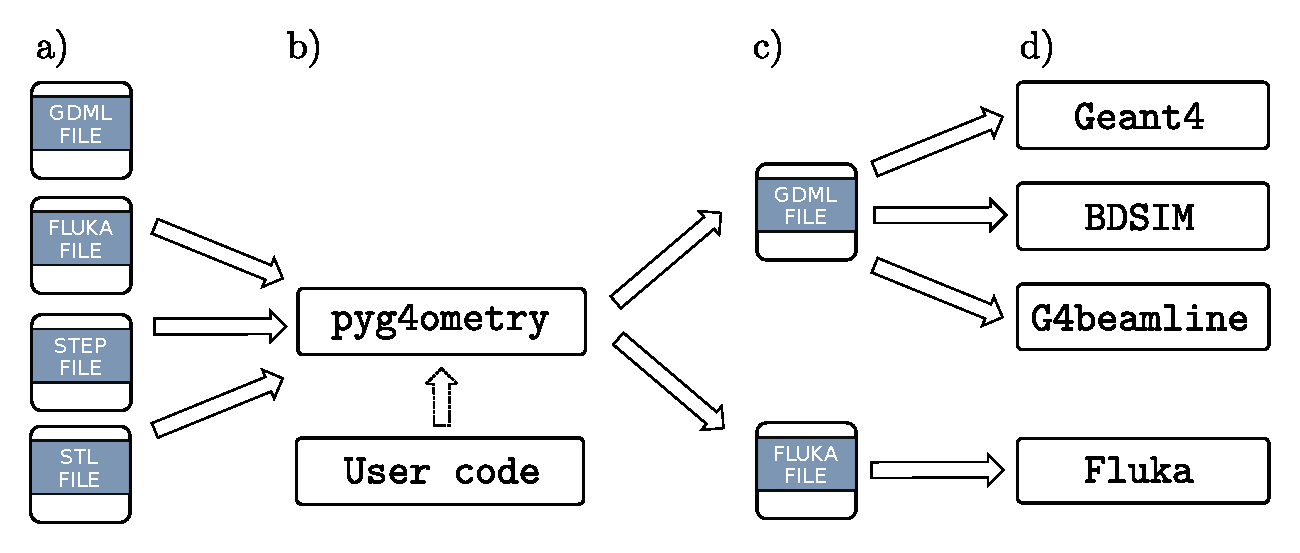
\includegraphics[width=0.7\textwidth]{./diagrams/workflow.pdf}
  \caption{\label{fig:workflow}Schematic of \PYGEOMETRY{} workflow, showing (a) the different input file formats, (b) Python processing, (c) output file targets and 
  (d) MCRT codes which use the geometry. }
\end{figure*}

There are existing codes that have functionality similar to \PYGEOMETRY{}. ROOT~\cite{Brun:1997pa}, the high-energy physics data analysis framework, 
can load, display and manipulate GDML-like geometry. Tools exist to convert CAD files to GDML, open source examples are GUIMesh \cite{GUIMesh_Pinto}, commercial 
products include ESABASE2~\cite{ESABASE2} and FASTRAD~\cite{FASTRAD}. There are also tools from the fusion and neutronics community that can convert CAD 
geometry into formats usable by MCRT codes, with examples including DAGMC~\cite{DAGMC} and McCAD~\cite{McCad}. In principle CAD software can export shape data to STL 
(or other similar mesh formats), which can be used by Geant4~\cite{poole2012acad}. In practice, using a lot of CAD models is difficult if that model is comprised of a 
large number of parts. Exporting, assigning material to, and placing the STL components into the MCRT code can be a cumbersome task. The existent set of software does not 
provide a complete set of tools to efficiently create complex geometries.

This paper is structured as follows, first a brief radiation transport-focused introduction to computer descriptions of geometry, followed by an explanation of the design 
and implementation of \PYGEOMETRY{}. The sections that follow describe how \PYGEOMETRY{} can be used to perform rapid geometric modelling, conversion from 
FLUKA to GDML, GDML to FLUKA and CAD to GDML. The paper concludes with an example of a composite, complex system consisting of components drawn from 
all the supported  geometry input files formats.

\section{Computer descriptions of geometry} \label{sec:geometric}
Central to a computer-readable geometry is how a solid is defined in three dimensions. There are numerous different ways to describe a
geometry, including constructive solid geometry (CSG), boundary representation (BREP) and tessellated polygons, which are described 
briefly in the following sections.  The Geant4 geometry specification is a mixture of geometry modelling techniques and described in detail last.

%%%%%%%%%%%%%%%%% Constructive solid geometry (CSG) 
Constructive solid geometry uses Boolean operations (subtraction, intersection and union), between simple solid shapes (e.g. cube, cylinder, sphere, etc.) or infinite
volumes (e.g. a plane-defined infinite half-space) to model complex surfaces which represent a solid. Boolean operations and solids can be combined to form a 
CSG tree to model complex geometry. FLUKA uses CSG to model solids, the form of Boolean expression used by FLUKA is not a general CSG tree but a 
logical expression in disjunctive normal form.

%%%%%%%%%%%%%%%%% Boundary representation (BREP)
Boundary representation consists of two parts, topology and geometry. Topological elements are faces, edges and vertices and the corresponding
geometrical elements are surfaces, curves and points. No current MCRT applications use native file formats employed by CAD systems. The conversion of 
CAD BREP formats for loading in MCRT applications is typically performed via a tessellated format, although it is possible to decompose BREP descriptions
 to bounded or infinite mathematical surfaces and subsequently solids as used in CSG descriptions. This type of conversion is complex and error-prone, 
 although recent progress has been made \cite{WangNuclSciTech31-82-2020}.

%%%%%%%%%%%%%%%%% Tessellated polygons
Solid volumes can be defined using triangular, quadrilateral or tetrahedral meshes. Numerous formats exist to describe meshes, the ubiquitous being STL with
more modern examples including PLY and OBJ. For solids with curved faces a tessellated mesh will always give an approximate description. As the mesh 
deviation distance from the solid decreases the number of polygons increases and with it the memory consumption and execution time of the MCRT simulation. 

%%%%%%%%%%%%%%%%% Geant4 geometery
Geant4 geometry description is a mixture of BREP, CSG and tessellated concepts. Geant4 includes 27 basic solids, although it does not store a sense 
of topology present in traditional CAD BREP systems. One of the fundamental solids is a tessellated solid which can be used to represent STL or PLY files. 
Geant4 also provides the ability to perform Boolean operations on these primitive solids. The richest and most flexible geometry description is currently used by
Geant4. Not only do solid objects need to be defined but also placed in a world coordinate system. Geant4 has two concepts which facilitate this \emph{logical volumes}
and \emph{physical volumes}. A logical volume is a region of space that is defined by an outer solid but also other attributes like material, magnetic field 
and zero or more \emph{daughter} physical volumes. A physical volume is a placement (or instance) of a logical volume. This design permits large reuse 
of objects, minimising memory footprint for largely repetitive structures such as detectors that Geant4 was created to simulate.  

%%%%%%%%%%%%%%%%% FLUKA geometry

%%%%%%%%%%%%%%%%% Geant Detector Mark-up Language
To exchange geometry descriptions between software packages the Geometry Description Markup Language (GDML) was developed~\cite{GDML}. 
GDML is an XML-based description of Geant4 geometry. Geant4 and ROOT~\cite{fons_rademakers_2019_3895860} can read and write 
GDML and it is commonly used as an exchange format for Geant4 geometries. 

\section{\PYGEOMETRY{} design and layout}
\PYGEOMETRY{} is a Python package consisting of semi-independent sub-packages. The sub-package \verb|pyg4ometry.geant4| contains all classes for 
Geant4 detector construction and \verb|pyg4ometry.gdml| provides the functionality for reading and writing GDML files. There are sub-packages for importing and 
exporting other geometry formats: \verb|pyg4ometry.fluka|, \verb|pyg4ometry.stl| and \verb|pyg4ometery.freecad|.  Lastly, the sub-package \verb|pyg4ometry.convert| 
is used for conversions between formats.

The core of \PYGEOMETRY{} consists of Python classes that mimic Geant4 solids, logical volumes, physical volumes, GDML parameters and material classes.
The constructors of the Python classes are kept as close to the original Geant4 C++ implementation as possible so that \PYGEOMETRY{} users do not have to learn 
a new API. For example the \verb|G4Box| class in Geant4, has the XML tag \verb|Box| in GDML and is represented by the \pyinline{Box} 
class in \PYGEOMETRY{}. The Python object initialisers are very similar to their corresponding Geant4 C++ constructors, but the length definitions are those used by GDML. For example, 
GDML uses full lengths whilst Geant4 uses half lengths. Geometry construction in Python proceeds in a way which is very similar to geometry construction in Geant4. 
A user relatively familiar with Geant4 should be able to start creating geometry in \PYGEOMETRY{} immediately. In the following sections novel or important developments 
in \PYGEOMETRY{} are described.  

%\begin{table}[hbt!]
%\centering
%\begin{tabular}{ l l l } \hline
%GDML tag 		& Child tags				& \PYGEOMETRY{} class 				\\ \hline
%Define 			& Constant				& gdml.Constant				\\
%				& Variable					& gdml.Variable					\\
%				& Quantity					& gdml.Quantity				\\
%				& Expression 				& gdml.Expression				\\
%				& Position					& gdml.Position					\\
%				& Rotation					& gdml.Rotation				\\
%				& Scale					& gdml.Scale					\\
%				& Matrix					& gdml.Matrix					\\ \hline
%Materials 		& Element					& geant4.Element				\\
%				& Isotope					& geant4.Isotope				\\
%				& Material					& geant4.Material				\\ \hline
%Solid  			& Box					& geant4.solid.Box				\\
%	  			& Tube					& geant4.solid.Tubs				\\
%	  			& CutTube				& geant4.solid.CutTubs			\\
%	  			& Cone					& geant4.solid.Cons				\\
%	  			& Para					& geant4.solid.Para				\\
%	  			& Trd					& geant4.solid.Trd				\\
%	  			& Trap					& geant4.solid.Trap				\\
%	  			& Sphere					& geant4.solid.Sphere			\\
%	  			& Orb					& geant4.solid.Orb				\\
%	  			& Torus					& geant4.solid.Torus				\\
%	  			& Polycone				& geant4.solid.Polycone			\\
%	  			& GenericPolycone			& geant4.solid.GenericPolycone	\\
%	  			& Polyhedra				& geant4.solid.Polyhedra			\\
%				& GenericPolyhedra                  & geant4.solid.GenericPolyhedra	\\ 
%	  			& Eltube					& geant4.solid.EllipticalTube		\\
%	  			& Ellipsoid					& geant4.solid.Ellipsoid			\\
%	  			& Elcone					& geant4.solid.EllipticalCone		\\
%				& Paraboloid				& geant4.solid.Paraboloid			\\
%				& Hype					& geant4.solid.Hyperboloid		\\
%				& Tet						& geant4.solid.Tet				\\
%				& Xtru					& geant4.solid.ExtrudedSolid		\\
%				& TwistedBox				& geant4.solid.TwistedBox		\\
%				& TwistedTtap				& geant4.solid.TwistedTrap		\\
%				& TwistedTrd				& geant4.solid.TwistedTrd 		\\
%				& TwistedTube				& geant4.solid.TwistedTube		\\
%				& Arb8					& geant4.solid.GenericTrap		\\
%				& Tessellated				& geant4.solid.TessellatedSolid 	\\
%				& Union					& geant4.solid.Union				\\
%				& Subtraction				& geant4.solid.Subtraction			\\
%				& Intersection				& geant4.solid.Intersection 		\\
%				& MultiUnion				& geant4.solid.MultiUnion 			\\
%				& ScaledSolid				& geant4.solid.ScaledSolid		\\				
%	  			& OpticalSurface			& geant4.solid.OpticalSurface		\\ \hline
%Structure		& Volume					& geant4.LogicalVolume			\\
%				& Assembly				& geant4.AssemblyVolume 		\\
%				& PhysVol					& geant4.PhysicalVolume			\\ 
%				& ReplicaVol				& geant4.ReplicaVolume			\\ 
%				& ParaVol					& geant4.ParameterisedVolume	\\ 
%				& DivisionVol				& geant4.DivisionVolume			\\
%				& SkinSurface				& geant4.SkinSurface			\\ 
%				& BorderSurface			& geant4.BorderSurface			\\ \hline
%
%\end{tabular}
%\label{tab:gdml-tags}
%\caption{GDML tags and corresponding \PYGEOMETRY{} classes.}
%\end{table}
    

%%%%%%%%%%%%%%%%%  Input and output  
For each input format available in \PYGEOMETRY{}  (GDML, STL, FLUKA and STEP) a dedicated \emph{Reader} class is implemented: \verb|gdml.Reader|,
\verb|stl.Reader|, \verb|fluka.Reader| and \verb|freecad.Reader|. Each reader constructs the appropriate Geant4 classes and provides a \verb|Registry| instance which 
can be used or manipulated by the user. 
Output consists of taking the registry and writing to file with the desired format.

%%%%%%%%%%%%%%%%%  Internal data representation
The internal data representation closely follows the structure of GDML. A \verb|Registry| class aggregates Python ordered dictionaries that are  used to store the main 
elements of a GDML file. As a \PYGEOMETRY{} user instantiates the geometry the registry is correspondingly updated. When a user is finished with the geometry, the registry 
can be written to disk as a GDML file. Multiple \verb|Registry| instances can be aggregated to form a composite geometry or volumes can be removed and added. 

%%%%%%%%%%%%%%%%%  Expression evaluation
In GDML symbolic expressions can be used to parametrise solids and their placement. These expressions are evaluated when the GDML is loaded into Geant4. 
In order to fully replicate the functionality of GDML an expression engine was implemented using ANTLR~\cite{10.5555/2501720}. The GDML is loaded using 
standard XML modules and parsed using ANTLR to create an abstract syntax tree (AST).  GDML allows for the definition 
and assignment of variables. GDML expressions are not much more complicated than binary operators $+, -, \times, /$ and common trigonometric and special 
functions $\sin, \cos, \tan$, etc. The AST terminates on either expressions which evaluate to numbers or GDML variables. Internally, all \PYGEOMETRY{} 
classes use GDML expressions and not floating-point numbers. Storing internal data as expressions allows for deferred evaluation (or re-evaluation) of 
solid parameters and  placements. This allows a user to update variables whilst defining geometry and the expression engine will update all internal values. 
An example of GDML expressions is shown in Listing~\ref{lst:gdmlExpressions}.

\begin{lstlisting}[caption={A simple Python script using \PYGEOMETRY{} to create GDML variables.},label={lst:gdmlExpressions}, language=Python]
# Import modules 
import pyg4ometry

# Create empty data storage structure
reg = pyg4ometry.geant4.Registry()

# Expressions 
v1 = pyg4ometry.gdml.Constant("v1","0",reg)
v2 = pyg4ometry.gdml.Constant("v2","sin(v1+pi)",reg)

\end{lstlisting}

 
%%%%%%%%%%%%%%%%%  Replica, division, parametrised and looped volumes
A powerful feature of Geant4 and hence GDML is the ability to either repeat, divide or parametrise geometry. The class which enables the creation of 
multiple replicas of a volume in a Cartesian, cylindrical or spherical grid is known as a Replica Volume. A Division Volume breaks a primitive into segments 
in either Cartesian or cylindrical polar coordinates. A parametrised volume allows for the arbitrary multiple placement of solids where the parameters are 
allowed to vary for each placement.  Another way in GDML to create parametrised solids or volumes is GDML loops, where sections of GDML can be 
 repeated with varying parameters based on the loop index. GDML loop loading and expansion are not supported by \PYGEOMETRY{} but will be implemented in a 
future release.
  
\subsection{Tessellation of solids (meshing)}
Creating a uniform three dimensional mesh description of all solids (including Booleans) is exceptionally useful for visualisation and other algorithms, such as overlap 
detection. For each Geant4 solid instance a triangular tessellated vertex-face mesh is generated and cached. This mesh is then used to determine the extent 
of placed instances of geometry (physical volumes) and meshes for CSG-derived solids. CSG mesh calculations are performed using a Binary Space Partitioning 
(BSP) tree technique in pure Python~\cite{pycsg} or the Computational Geometry Algorithms Library (CGAL) surface meshes \cite{cgal:bsmf-sm-20b} in C++. In 
general the CGAL implementation is one to two orders of magnitude faster than the pure Python CSG implementation and must be used for large geometries. 
Triangular meshes based on CSG operations involving curved surfaces often contain large numbers of triangles. Before meshes are visualised or written to file 
various polygon mesh algorithms  from CGAL \cite{cgal:lty-pmp-20b} can be employed to give the meshes more desirable features. 

%%%%%%%%%%%%%%%%% Volume bounding
If a user is creating and placing multiple daughter volumes within a \emph{mother} volume then it is the user's responsibility to create a solid which fully 
encompasses the daughter volumes. Overlaps between daughter volumes and the mother can be detected, but it is desirable 
% \colorbox{yellow}{It's not just desirable, it's absolutely necessary isn't it?  And I'm not sure what the word ``efficiently'' means precisely in this context.} 
to have a mother volume shape that efficiently holds its daughters. However, there are exceptions to this rule in the form of assembly volumes. 
 
\subsection{Visualisation} \label{sec:visualisation}
When implementing geometry a rapid and robust visualisation system is key to produce error-free and efficient simulation input.
A  \PYGEOMETRY{} geometry hierarchy can be viewed using the popular Visualisation Toolkit (VTK). No separate scene graph is required as the Geant4 
volume hierarchy is sufficient to place the meshes associated with each physical volume. A daughter volume is placed within a logical volume with a rotation 
$\mathbf{R}_d$, scale $\mathbf{S}_d$ and translation $\mathbf{T}_d$.

\begin{figure}[htb!]
\begin{center}
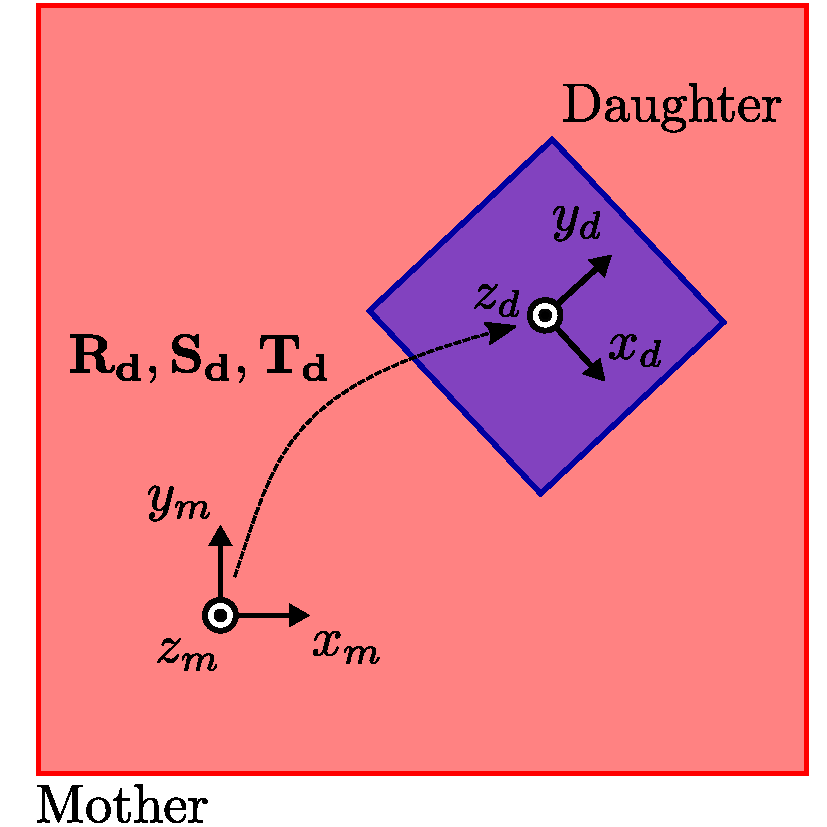
\includegraphics[width=5cm]{./diagrams/lvToPv.pdf}
\caption{The placement of a physical volume inside a logical volume.}
\label{fig:lvToPv}
\end{center}
\end{figure} 

The transformation  $\mathbf{M}$  and translation $\mathbf{T}$ from mother to daugher is 
\begin{eqnarray}
\mathbf{M} 	& = &  \mathbf{S}_d  \mathbf{R}_d\,, \\
\mathbf{T} 	& = &  \mathbf{T}_d\,.
\end{eqnarray}
%
If the mother volume is placed in the world then the placement transformation $\mathbf{M}_w$ and translation $\mathbf{T}_w$ are expressed as
\begin{eqnarray}
\mathbf{M}_w	  	& = & \mathbf{M}_m \mathbf{M}_d  = \mathbf{S}_m \mathbf{R}_m  \mathbf{S}_d \mathbf{R}_d\, ,				\label{eqn:worldToDaughter1}\\
\mathbf{T}	_w 		& = & \mathbf{M}_m \mathbf{T}_d + \mathbf{T}_m= \mathbf{S}_m \mathbf{R}_m \mathbf{T}_d + \mathbf{T}_m\,,  \label{eqn:worldToDaughter2}
\end{eqnarray}
where the subscript $m$ indicates mother volume and $d$ indicates daughter volume. Given a hierarchy of logical and physical volumes, 
Equations~\ref{eqn:worldToDaughter1} and \ref{eqn:worldToDaughter2} can be used recursively to place an arbitrary number of nested volumes.

The physical volume class (\pyinline{pyg4ometry.geant4.PhysicalVolume}) is also used to store visualisation attributes like the solid's 
colour, surface or wireframe representation and visibility. Overlaps detected in the mesh geometry are
stored in the Logical Volume and can be  displayed separately to allow a user to visually identify and debug the the overlaps.   

%%%%%%%%%%%%%%%%% Adding properties to volumes
Geometry needs to be augmented with other information for a complete MCRT simulation. Often other attributes need to be 
assigned to regions of space, for example material definition, magnetic field or optical properties. These physical properties 
can be used to define the visualisation attributes of a volume. 

\subsection{Overlap detection}
All MCRT codes cannot handle spatial overlap between two geometric objects and will have ill-defined behaviour when tracking particles  
in such a situation.  A key feature of \PYGEOMETRY{} is the detection of potential overlaps in a way which is most useful to the user, it does this by 
performing an intersection operation between solid instances and determining if the resultant mesh is empty. Figure~\ref{fig:overlap} shows the potential 
overlaps, (a) protrusion of a daughter from the mother, (b)  finite volume intersection between two daughters  and (c) an overlap where two daughters 
share a face. If the resulting intersection is non-null then the overlaps can be displayed side-by-side in the visualisation. 
\begin{figure}[htbp]
\begin{center}
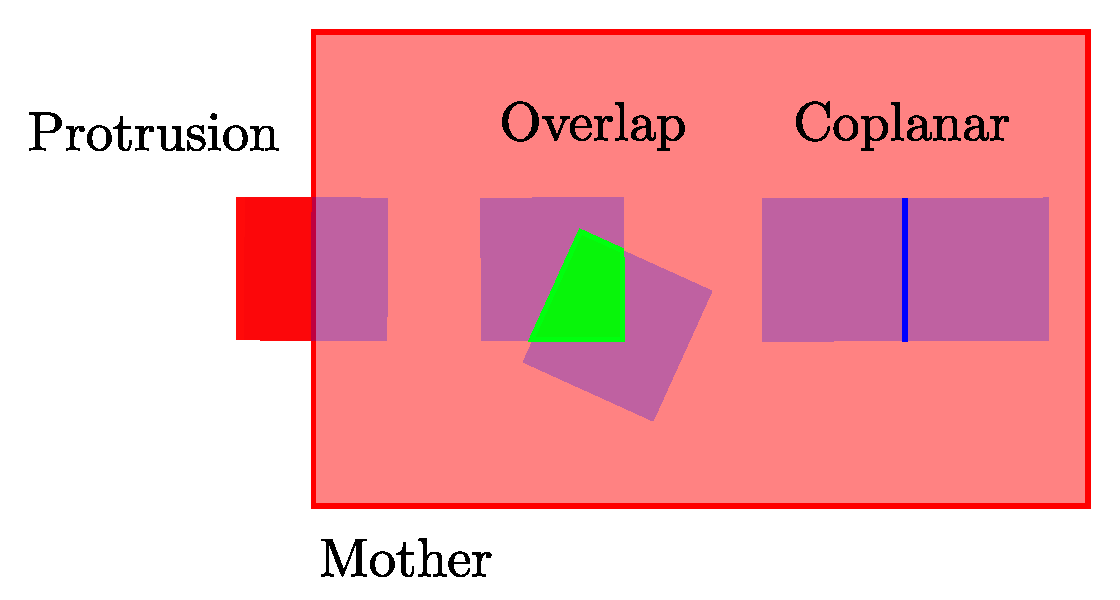
\includegraphics[width=8cm]{./diagrams/overlap.pdf}
\caption{Schematic of the three different types of overlap between daughters of a mother logical volume.}
\label{fig:overlap}
\end{center}
\end{figure} 


\begin{algorithm}[h]
  \SetKwProg{Int}{Function}{}{}
  \SetKwFunction{Intersection}{Intersection}%
  \SetKwProg{OCheck}{Function}{}{}
  \KwData{Logical volume $v$ with mesh $m$ and daughter volume meshes $d\in D$.}
  \KwResult{Set $S$ of non-null mesh intersections.}
  
  % Define the function used in the algorithm
  \Int{\Intersection{$n_1, n_2$}}{
    \KwData{CSG meshes $n_1$ and $n_2$.}
    \KwResult{The mesh intersection of $n_1$ and $n_2$.}
  }
  % The actual algorithm
  $V \longleftarrow \emptyset$\tcp*[r]{Cache tried mesh pairs.}
  $S \longleftarrow \emptyset$\;
  
  \For{$d_1 \in D$}{
    $p \longleftarrow$ \Intersection{$m,d_1$}\;
    \If{$p$ is not null}{
      $S \longleftarrow S \cup \{p\}$\;
    }
    \For{$d_2 \in D$}{
      \If{$d_1 = d_2$ {\bf or} $(d_2, d_1) \in V$}{
        \textbf{continue}\;
      }
      $q \longleftarrow \Intersection{a,b}$\;
      \If{$q$ is not null}{
        $S \longleftarrow S \cup \{q\}$\;
      }
      $V \longleftarrow V \cup \{(d_1, d_2)\}$\;
    }
  }
  \label{algo:overlap}
  \caption{The overlap checking algorithm employed in \PYGEOMETRY{}.}
\end{algorithm}

Overlap detection in \PYGEOMETRY{} relies of the meshes generated for each solid, 
any detection algorithm will be approximate. Generally the overlap detection 
algorithm proceeds as shown in Algorithm~\ref{algo:overlap}.

For a logical volume with $n_{\rm daughters}$ physical volumes, assuming meshes for solids have an average number of faces $n$, clearly this algorithm 
has complexity $\sim \mathcal{O}(n^2 n_{\rm daughters}^2)$. This might seem like a prohibitive computational cost, but worth it considering the potential 
waste if small overlaps are present in the final MCRT simulation and large amounts of cluster CPU time is wasted. This algorithm clearly favours geometry 
descriptions which have a high degree of logical volume reuse. Due to the discrete nature of triangular meshes it is not possible to have perfect detection 
of overlaps, especially when curved surfaces are considered. The deviation of the meshes created from a solid can be controlled by the user reducing the 
chances of missing a potential overlap, but the algorithm presented here cannot capture all overlap cases. The overlap detection algorithm can 
present the potential overlaps quickly and easily to the user, thus significantly aiding their modelling process. 

\section{Rapid geometry modelling}
Given the Python scripting interface, expression  and tessellation engines it is possible for a user to rapidly specify the geometrical layout of the RT problem, vary 
the parameters of the geometry and visualise it.  When a user has achieved the desired geometry, without geometry overlaps, a GDML file can be written to file 
from the internal memory representation. Some example code is presented in Listing~\ref{lst:pythonRapidModelling}. The structure should be familiar to regular 
users of Geant4 or GDML, apart from the new class described in the previous section called the \pyinline{Registry}. First the \verb|Registry| is created to store all 
the \PYGEOMETRY{} objects; followed by constants;  then materials and properties, solids and logical and physical volumes; finally the whole geometry can be saved
as a GDML file or visualised using VTK.

\begin{lstlisting}[caption={A simple Python script using \PYGEOMETRY{} to create a simple Geant4 geometry.},label={lst:pythonRapidModelling}, language=Python]
# import modules 
import pyg4ometry.gdml as gd
import pyg4ometry.geant4 as g4
import pyg4ometry.visualisation as vi

# create empty data storage structure
reg = g4.Registry()

# expressions
wx = gd.Constant("wx","100",reg)
wy = gd.Constant("wy","100",reg)
wz = gd.Constant("wz","100",reg)
bx = gd.Constant("bx","10",reg)
by = gd.Constant("by","10",reg)
bz = gd.Constant("bz","10",reg)
br = gd.Constant("br","0.25",reg)

# materials
wm = g4.MaterialPredefined("G4_Galactic")
bm = g4.MaterialPredefined("G4_Fe")

# solids
wb = g4.solid.Box("wb",wx,wy,wz,reg)
b  = g4.solid.Box("b",bx,by,bz,reg)

# structure
wl = g4.LogicalVolume(wb, wm, "wl", reg)
bl = g4.LogicalVolume(b, bm, "b", reg)
bp1 = g4.PhysicalVolume([0,0,0],
                        [0,0,0],
                        bl, "b_pv1", wl, reg)
bp2 = g4.PhysicalVolume([0,0,-br],
                        [-2*bx,0,0],
                        bl, "b_pv2", wl, reg)
bp3 = g4.PhysicalVolume([0,0,2*br],
                        [2*bx,0,0],
                        bl, "b_pv3", wl, reg)

# define world volume
reg.setWorld(wl.name)

# physical volume vistualisation attributes
bp1.visOptions.color = (1,0,0)
bp1.visOptions.alpha = 1.0
bp2.visOptions.color = (0,1,0)
bp2.visOptions.alpha = 1.0
bp3.visOptions.color = (0,0,1)
bp3.visOptions.alpha = 1.0

# gdml output
w = gd.Writer()
w.addDetector(reg)
w.write("output.gdml")

# visualisation
v = vi.VtkViewer(size=(1024,1024))
v.addLogicalVolume(wl)
v.addAxes()
v.view()
\end{lstlisting}

An example of the VTK output for code
Listing~\ref{lst:pythonRapidModelling} is shown in
Figure~\ref{fig:rapidModellingExample}. Significantly more complex
geometries can be developed using a structure similar to that shown.

\begin{figure}[htbp]
\begin{center}
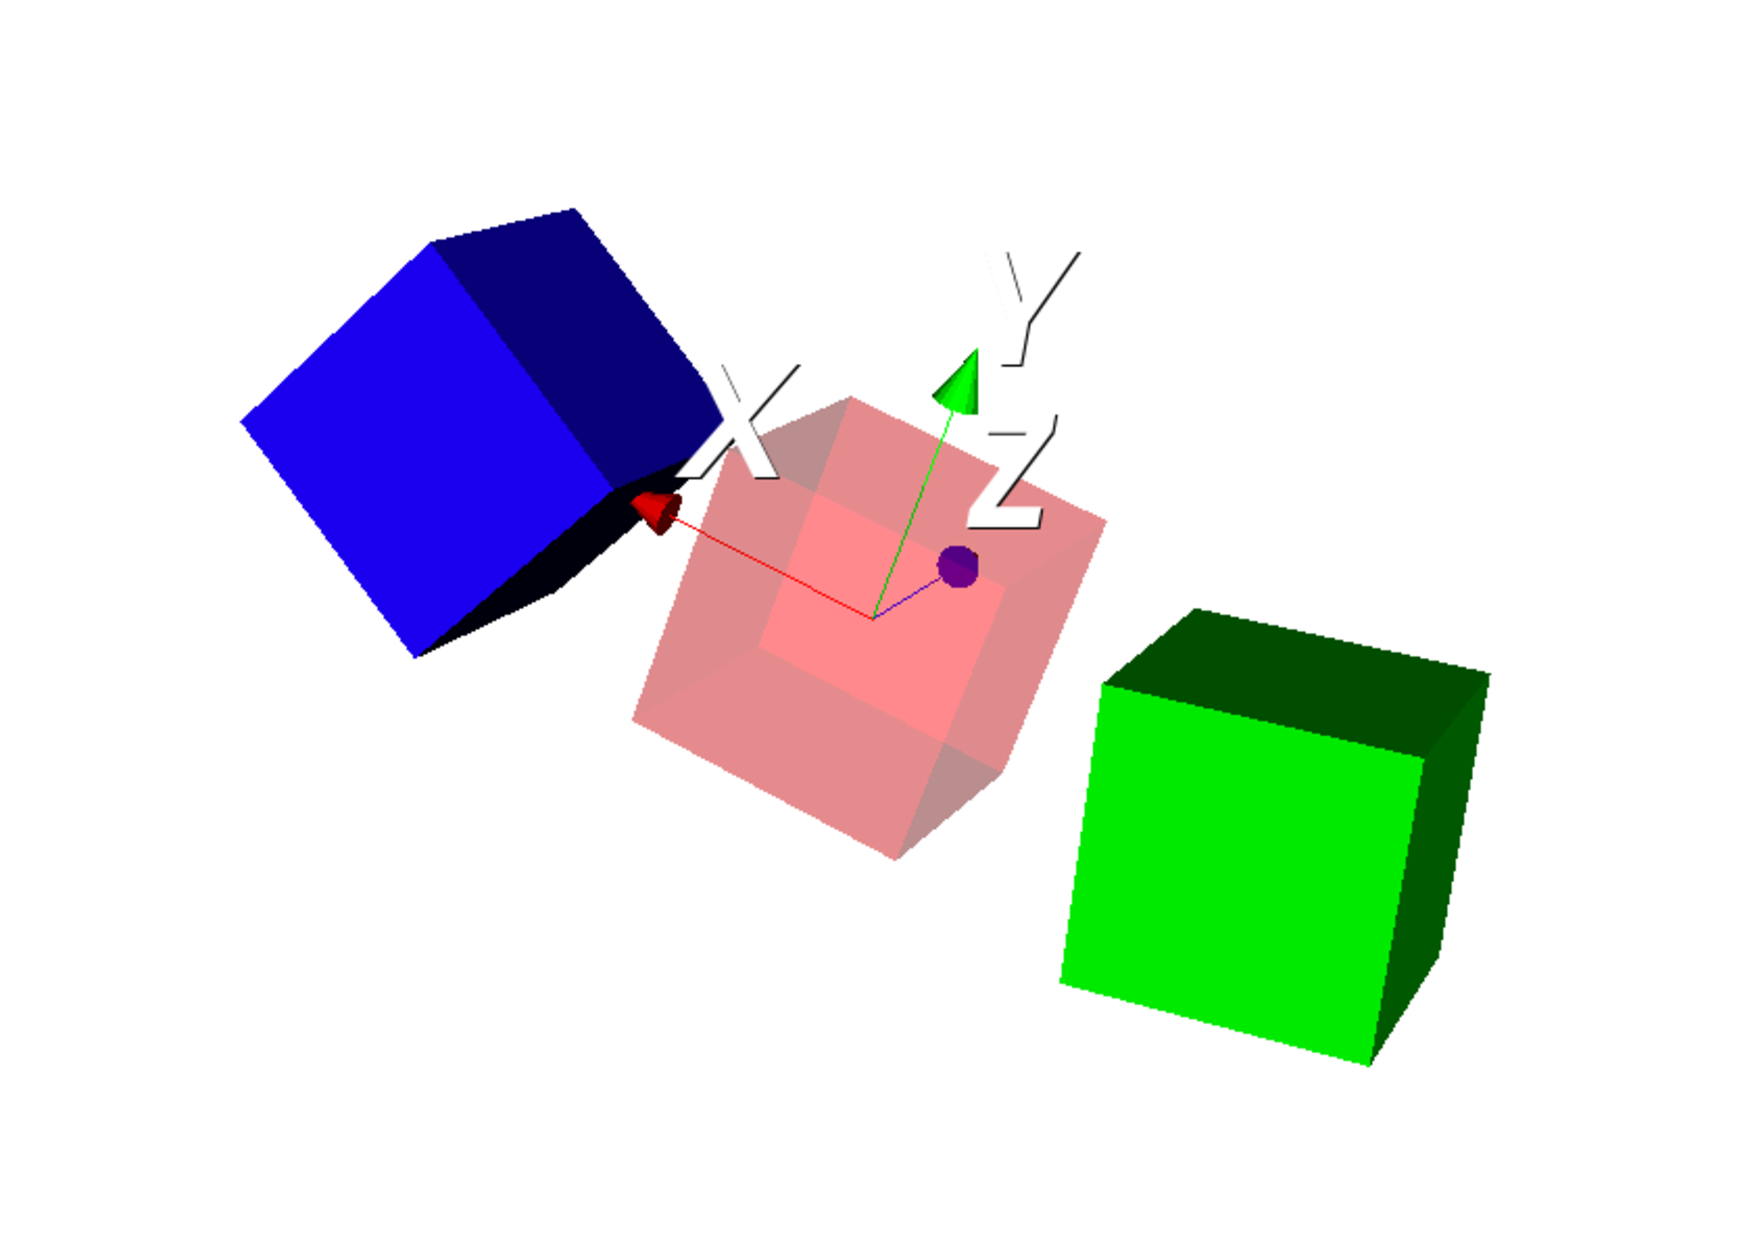
\includegraphics[width=0.9\columnwidth]{./diagrams/rapidModelling.pdf}
\caption{VTK visualisation output from code Listing~\ref{lst:pythonRapidModelling}.}
\label{fig:rapidModellingExample}
\end{center}
\end{figure}

The \PYGEOMETRY{} Python code in the example is approximately as expressive 
as the GDML it writes. The benefit of wrapping GDML/Geant4 in Python allows 
to very rapid prototyping of geometry without concerns of compilation of C++ (in the 
case of Geant4) or writing well formed XML (in the case of GDML). Effectively
the Python interpreter checks input for syntax errors when using \PYGEOMETRY{} classes. 
Another key benefit is the ability to use the \PYGEOMETRY{} code to create 
programmatic converters between different geometry languages or more generally 
manipulation and transformation of the geometry stored in memory. The rapid modelling 
example given in Listing~\ref{lst:pythonRapidModelling} and Figure~\ref{fig:rapidModellingExample} 
is rather trivial, a significantly more complex example is shown in Figure~\ref{fig:gdml-flair}.

\section{FLUKA to GDML conversion}
FLUKA geometry is based upon a limited set of primitives (referred to as
\emph{bodies}) which can be combined using Boolean operations. A
\emph{zone} consists of one or more bodies or \emph{subzones} combined
using intersections and subtractions.  Zones may then be further combined
using union operations to form \emph{regions}, which is defined as the
union of one or more zones, as well as a material.

\begin{figure}[htbp]
\begin{center}
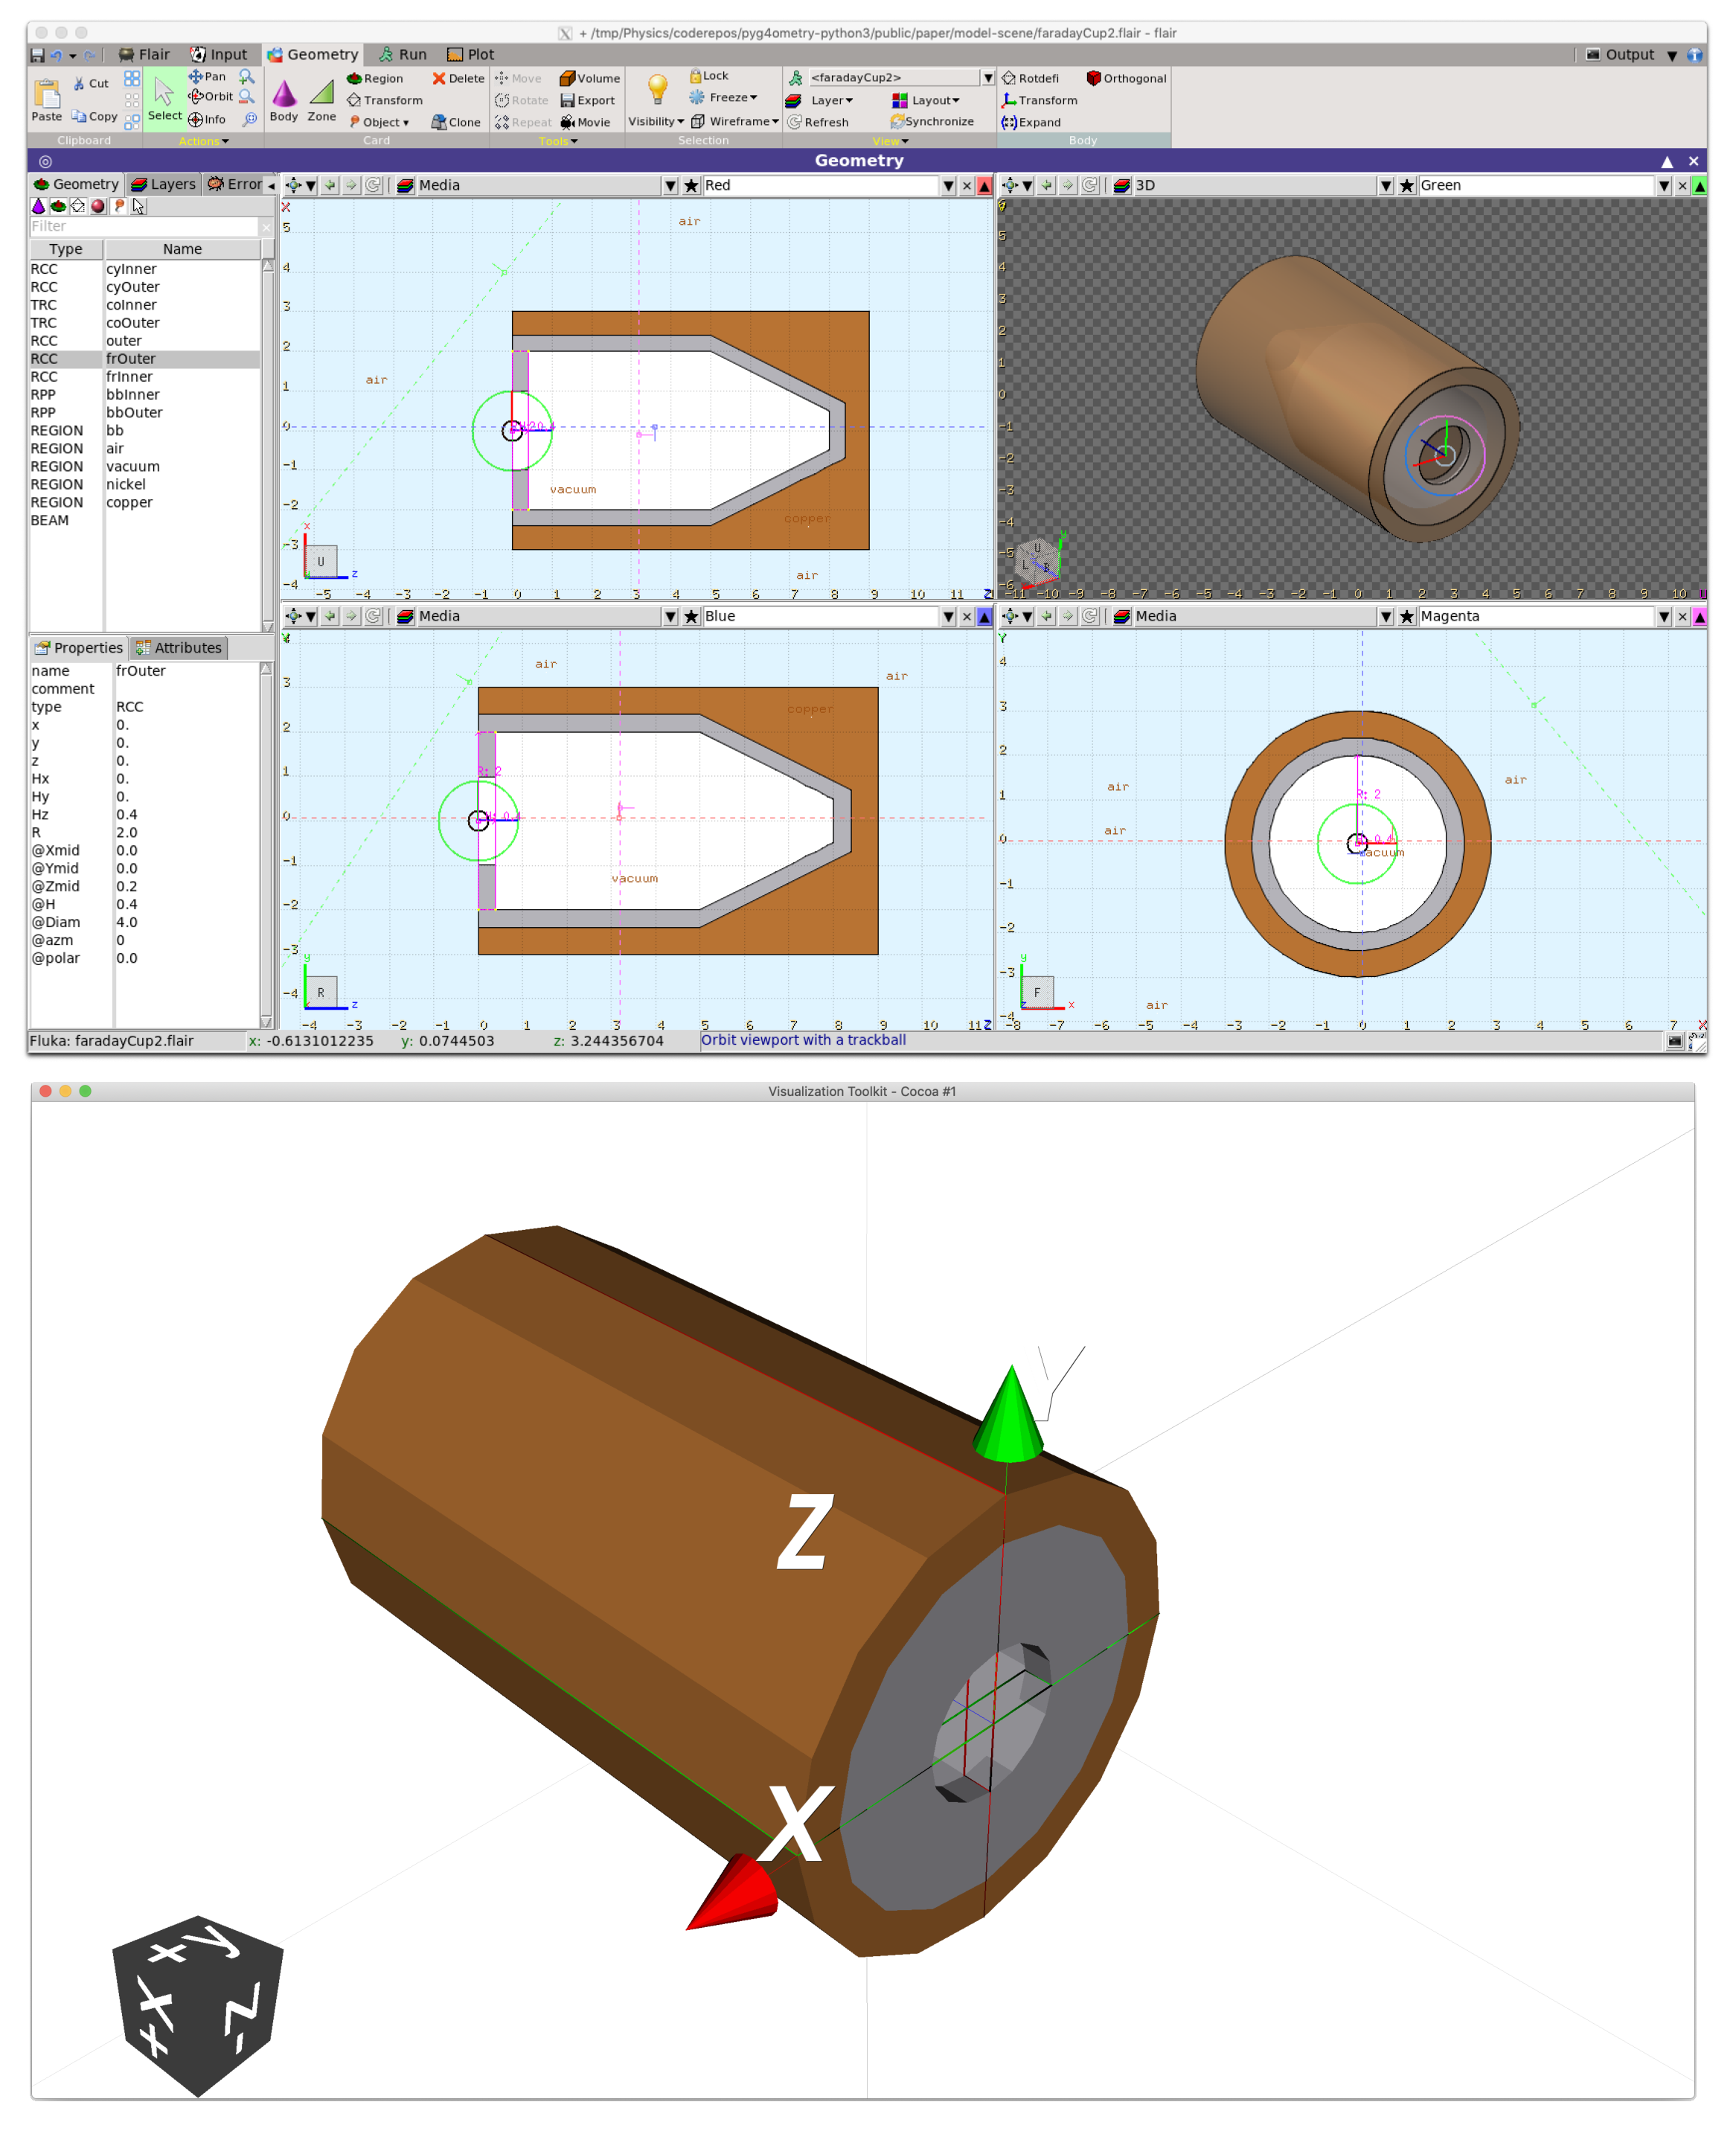
\includegraphics[width=0.9\columnwidth]{./model-scene/faradayCup2.pdf}
\caption{Example conversion of a simple FLUKA geometry to GDML. Above:
the original FLUKA geometry displayed in flair. Below: the GDML geometry
viewed in \PYGEOMETRY{}. The example is a Faraday cup used to capture
and measure accelerator beam charge.}
\label{fig:fluka-to-geant4-cup}
\end{center}
\end{figure}

Each FLUKA body is represented in \PYGEOMETRY{} with a corresponding
class, and in turn each class has methods which returns a GDML
primitive solid and that solid's rotation and position such that it
matches its FLUKA equivalent.  The expansion, translation and
transform geometry directives are each folded into one or more of
these three methods.  The mapping of FLUKA bodies to GDML solids is
shown in Table~\ref{tab:Fluka2Geant4}.  It is worth noting that many
of the FLUKA bodies are infinite in extent, but are mapped to finite
GDML solids.  The translation of infinite bodies to equivalent finite
solids is one of the main steps involved in the conversion process.
This mapping is possible because whilst FLUKA bodies can be infinite
in extent, all zones and regions must be finite.  Zones and regions
are then composed by instantiating these classes and adding body
instances to them.  Each zone and region instance can then return its
equivalent GDML Boolean solid.

The FLUKA CSG ASCII format is parsed using an ANTLR4-generated parser,
producing an AST.  The resulting AST is then inspected sequentially (walked)
to populate Region instances with zones and bodies.  With the region
instances populated they can then be manipulated and translated into GDML.
The translation involves a number of special steps to bridge the two
disparate formats and ensure the resulting GDML is well-formed and usable
in Geant4.  Some of these steps are simple, for example in FLUKA unions can
be disconnected, but in Geant4 specifically only MultiUnions can be
disconnected, such that MultiUnions are used throughout the converted
geometry instead of the usual binary unions.  Other procedures are more
involved and are discussed in the rest of this section.

\begin{lstlisting}[caption={A simple \PYGEOMETRY{} Python script to load a FLUKA file.},label={lst:pythonFlukaLoading}, language=Python]
    reader      = pyg4ometry.fluka.Reader("FlukaFileName.inp")
    g4_reg     = pyg4ometry.convert.fluka2Geant4(reader.flukaregistry)
    logical      = g4_reg.getWorldVolume()
\end{lstlisting}


\begin{table}[hbt!]
\caption{FLUKA bodies and their corresponding Geant4 solids.} \label{tab:Fluka2Geant4}
\centering
\begin{tabular}{ll} \hline
FLUKA body                                              & \PYGEOMETRY{} class \\ \hline
RPP (Rectangular parallelepiped)			& Box \\
BOX (General rectangular parallelepiped)		& Box \\
SPH (Sphere)    					& Orb \\
RCC (Right circular cylinder)				& Tubs \\
REC (Right elliptical cylinder)				& EllipticalTube \\
TRC (Truncated Right Angle Cone)			& Cons \\
ELL (Ellipsoid of Revolution) 				& Ellipsoid \\
WED/RAW (Right Angle Wedge)		        	& ExtrudedSolid \\
ARB	(Arbitrary Convex Polyhedron)			& TessellatedSolid \\
XYP 	($X$-$Y$ Infinite half-space)			& Box \\
XZP 	($X$-$Z$ Infinite half-space)			& Box \\
YZP 	($Y$-$Z$ Infinite half-space)			& Box \\
PLA (Generic infinite half-space)			& Box \\
XCC ($X$-axis Infinite Circular Cylinder)		& Tubs \\
YCC ($Y$-axis Infinite Circular Cylinder)		& Tubs \\
ZCC 	($Z$-axis Infinite Circular Cylinder)		& Tubs \\
XEC 	($X$-axis Infinite Elliptical Cylinder)		& EllipticalTube \\
YEC 	($Y$-axis Infinite Elliptical Cylinder)		& EllipticalTube \\
ZEC ($Z$-axis Infinite Elliptical Cylinder)		& EllipticalTube \\
QUA (Quadric surface) 					& TessellatedSolid \\ \hline
\end{tabular}
\end{table}

\subsection{Infinite bodies}
The majority of bodies in FLUKA are infinite in extent, and fall
broadly into four categories, half-spaces, infinitely long cylinders,
infinitely long elliptical cylinders and quadric surfaces.
Translating these bodies to Geant4 requires generating the equivalent
finite solid whilst retaining the same final finite Boolean shape.
This is achieved with the use of axis-aligned bounding boxes (AABB),
in which the FLUKA body is translated to a finite solid with with
dimensions slightly larger than the AABB.  The lengths of infinite
(elliptical) cylinders are reduced to finite equivalents with lengths
slightly greater than the bounding box.  Similarly, half spaces are
reduced to boxes with one face acting as that of the half-space face,
and quadric surfaces are sampled only over the volume denoted by the
AABB.  Furthermore, the positions of these solids are moved as close
to the bounding box as possible whilst retaining an identical final
Boolean geometry.

Generating these bounding boxes over which the bodies should be
translated involves first evaluating each region with very large Tubs,
EllipticalTubes and Boxes (by default \SI{50}{\km} in length), such
that they are effectively infinite for most reasonable use cases.
\PYGEOMETRY{}'s CSG meshing is then used to generate a mesh for each
region, from which the axis-aligned bounding box can be extracted.
Each region is then evaluated a second time with respect to its
respective bounding box, with all of its constituent infinite solids
being reduced as described above.  This algorithm works robustly for
infinite (elliptical) cylinders and half spaces as the number of
facets is independent of the size of the solid, so generating the
initial mesh from large solids works well.  Generating a quadric
surface over a very large volume in space whilst retaining topological
information is computationally very expensive, so to resolve this the
user must provide the approximate axis-aligned bounding box of any
region in which a quadric is used.

\subsection{Removing redundant half-spaces}
The above algorithm for replacing infinite FLUKA bodies with finite
Geant4 solids works well in most cases, but additional care must be
taken for redundant infinite half spaces.  A redundant infinite half
space is defined as one which has no affect on the topology of the
final Boolean solid.  Whilst this may be true of arbitrary bodies, it
is most problematic for half spaces as after the infinite-body
reduction has been performed, if the half-space is far away from the
region's AABB, then it can result in a malformed Boolean.  This algorithm is
demonstrated in Algorithm~\ref{algo:redundant-halfspace}.  Such
half-spaces are filtered from their respective regions during the
conversion process by calculating the nearest distance from the centre
of the AABB to the half-space face.  If this distance is greater than
the centre-to-corner distance of the AABB, then that half-space is
removed from the region during conversion.

\begin{algorithm}

  \KwData{FLUKA regions to be converted to GDML.}
  \KwResult{GDML solids equivalent to the FLUKA regions built from
    minimally-sized primitive solids}

  \SetKwProg{ToGDML}{Function}{}{}
  \SetKwFunction{ToGDMLSolid}{ToGDMLSolid}

  % The function for translating a fluka body to a finite GDML solid.
  \ToGDML{\ToGDMLSolid{$b, a$}}{
    \KwData{FLUKA body $b$ with axis-aligned bounding box $a$.}
    \KwResult{GDML solid equivalent to $b$ bounded by the volume $a$.}
  }

  \SetKwProg{RAABB}{Function}{}{}
  \SetKwFunction{RegionAABB}{RegionAABB}
  % The function for translating a fluka body to a finite GDML solid.
  \RAABB{\RegionAABB{$r$}}{
    \KwData{FLUKA region $r$.}
    \KwResult{Axis-aligned bounding box (AABB) of the FLUKA region.}
  }

  $ B \longleftarrow \emptyset$\tcp*[r]{Map of regions to AABBs.}
  \For{$r$ in regions to be converted}{
    $B[r] \longleftarrow$ \RegionAABB{$r$}
  }

  \tcp{Map of bodies to minimal bounding boxes.}
  $ E \longleftarrow \emptyset$\;
  \For{$b$ in bodies in regions to be converted}{
    \For{$r$ in regions in which body $b$ is used}{
      $E[b] \longleftarrow E[b] \cup $ \RegionAABB($r$)\;
    }
  }

  $ G \longleftarrow \emptyset$ \;
  \For{body $b$ and AABB $a$ in $E$}{
    \tcp{Map the fluka bodies to minimal GDML solids by converting with the
    minimal AABB, $a$.}
    $G \longleftarrow $ \ToGDMLSolid{$b, a$}\;
  }
  \For{$r$ in regions to be converted}{
    build the corresponding GDML for $r$ from the set of minimal GDML
    primitives in $G$.\;
  }

  \label{algo:redundant-halfspace}
  \caption{The infinite-body minimisation algorithm employed in the
    conversion of Fluka to GDML.}
\end{algorithm}

\subsection{Coplanar faces}
Coplanar faces, in which the faces of two union components or that of
two regions are perfectly coplanar in FLUKA are ubiquitous and present
no difficulties to the operation of the program.  However, in Geant4
these will generally result in tracking errors.  These must be handled
robustly to ensure the resulting geometry is usable.  Coplanar faces
are resolved automatically by slightly decreasing the size of every
body that is used in an intersection, and increasing the size of every
body used in a subtraction.  These rules are inverted for nested
subtractions and work well for guaranteeing well-formed geometry that
is free from overlaps.

\subsection{Materials}

Any useful translation between geometry description formats must also
account for material, and accordingly \PYGEOMETRY{} correctly translates
FLUKA materials to GDML.  FLUKA materials can be divided into built-in ,
single-element and compound materials.  Built-in materials are simply those
that are predefined by FLUKA, single-element materials are described with a
single \fluka{material} card, and compound materials are described with one
\fluka{material} card followed by one or more \fluka{compound} cards.
These three alternatives are represented in \PYGEOMETRY{} with the
\pyinline{BuiltIn}, \pyinline{Material}, and \pyinline{Compound} classes.
Populating a hierarchy of instances using these classes is involved due to
the fact that recursively-defined materials in FLUKA input files need not
be defined in a logical order.  Namely, a given \pyinline{compound} may be
defined before the materials that it consists of are themselves defined.
To account for this it is necessary to correctly compute the instantiation
order so that the above classes and be instantiated correctly.  To do this
a directed acyclic graph is populated with the materials and their
constituents, after which a topological sort is performed so that the
compound materials are sequenced after their constituents.  Mapping this
set of nested FLUKA material instances to GDML material instances is then
straight forwards as the GDML material semantics are slightly more
expressive than FLUKA's, so a one-to-one mapping is trivial.


\subsection{Lattice}

FLUKA supports modular geometries with the use of the \fluka{lattice}
command. Figure~\ref{fig:lattice} demonstrates this capability, and. The
arbitrarily complex \emph{basic unit} can be defined once and used
multiple times by placing one or more empty \emph{lattice cells} with the
associated roto-translation from that \fluka{lattice} cell to the basic
unit. The \fluka{lattice} cells themselves will generally lack structure
and simply serve as a reference to the basic unit. The rototranslated
lattice cell must fully contain the basic unit and all of the regions
within it. When a particle steps into the \fluka{lattice} cell, the
rototranslation is applied to that particle and it is is taken into the
basic unit, and the simulation continues within the basic unit. Any
particles leaving the basic unit will be translated back to the
\fluka{lattice} cell with the inverted rototranslation. Up to two
levels of \fluka{lattice} nesting the are supported in FLUKA.

\begin{figure}[hbtp]
\begin{center}
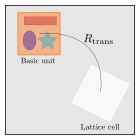
\includegraphics[width=6cm]{./diagrams/lattice}
\caption{The \fluka{lattice} feature demonstrating a \fluka{lattice} cell
  referring to its basic unit with the rototranslation $R_\textrm{trans}$.
  Any particle entering the cell will be transformed onto the basic unit
  with $R_\textrm{trans}$, and when leaving the basic unit, back to the cell
  with $R_\textrm{trans}^{-1}$.}
\label{fig:lattice}
\end{center}
\end{figure}

This feature is clearly analogous to the logical/physical volume feature in
Geant4, although it is less explicit as the contents of a given logical
volume are clearly stated, whereas the contents of a \fluka{lattice} cell
are implied by the combination of the rototranslation and the locations of
its \fluka{lattice} cell and basic unit.

Translating this construct into a logical volume (basic unit) with many
physical volumes (\fluka{lattice} cells) requires associating each
\fluka{lattice} cell with the full contents of its corresponding basic unit
(typically several regions). This is achieved by meshing the complete
FLUKA geometry and then rototranslating the \fluka{lattice} cell mesh with
its associated rototranslation. By construction this will translate the
\fluka{lattice} cell mesh directly onto the full basic unit mesh. Finally,
in checking for overlaps, the regions within the the basic unit can be
determined. In the final conversion step, the \fluka{lattice} cell can
simply be replaced with a physical volume that refers back to logical
volumes located in the previous step. Thus the \fluka{lattice} cells can
be translated into Geant4's logical/physical volumes. As has been stated,
FLUKA supports two levels of nesting, but currently the conversion to GDML
supports only one. However, extending to an extra level is simple in that
it only involves an extra application of a rototranslation matrix before
checking for overlaps.

\subsection{Discussion}

Figure~\ref{fig:fluka-to-geant4-cup} shows a Faraday cup implemented in
FLUKA and accurately translated to GDML using \PYGEOMETRY{}.  Many of the
steps described above were directly applied in this model and all the
features are tested and demonstrated in the repository.  This set of
algorithms for bridging FLUKA with GDML covers a very broad range of
geometries, however a number of possible improvements for the future
persist.  For example, Boolean solids in FLUKA can in general be
disconnected, and this most typically manifests itself in the form of
disconnected unions, but is also allowed for intersections and
subtractions.  Disconnected unions are readily available in GDML with the
use of the MultiUnion solid type, however there is no valid means to
construct a disconnected subtraction or intersection in GDML.  One possible
solution would be to detect these two cases, and if found, split them into
their constituent parts and place separately as TesselatedSolid instances.

Furthermore, the quadric surface conversion can be further improved by
specialising on some of the individual forms of the quadric.  Simply
converting every quadric into a TesselatedSolid comes at a potential
performance cost in the tracking, as well as usability in \PYGEOMETRY{} as the
user must provide an AABB.  In some cases tessellation in unavoidable (for
example a hyperbolic paraboloid), but parabolic cylinders could for example
be translated to an ExtrudedSolid.  This could provide both a performance
improvement in the tracking time and make \PYGEOMETRY{} easier to use as an
AABB would not need to be provided beforehand.  This has not been
implemented as quadrics are relatively rarely used, but where quadrics are
used its often parabolic cylinders (e.g. magnet pole tips) this
specialisation in particular would be worth implementing.

\section{GDML to FLUKA conversion}
It is relatively straight forward to convert Geant4 geometry to FLUKA. Each
of the Geant4 solids can be mapped to a FLUKA region.  A region is a region
of space defined by a material and the Boolean disjunction (a union using
the operator~$\:|\:$ in free format geometry) of one or more
zones. Each zone is then defined in terms of the conjunction (intersection
with~$+$, subtraction with~$-$) of one or more primitive bodies, as well as
parentheses to determine the order of operations within the zone.  FLUKA
has 20 of these primitive bodies, listed in Table~\ref{tab:Fluka2Geant4}
and, in general, infinite extent bodies have tracking accuracy and
efficiency benefits over finite ones. Key for conversion are XY-, XZ-,
YZ-Planes (XYP, XZP, YZP), arbitrary plane (PLA), Z-axis aligned cylinder
(ZCC), Z-axis aligned elliptical cylinder (ZEC), sphere (SPH), truncated
right-angle cone (TRC) and general quadric surface (QUA). Some solids in
Geant4 directly map to a single FLUKA body, others require the construction
of a simple FLUKA CSG tree combining these
primitives. Table~\ref{tab:geant2fluka} lists the mapping between Geant4
solids and the bodies used to compose a FLUKA region.
\begin{figure}
\begin{center}
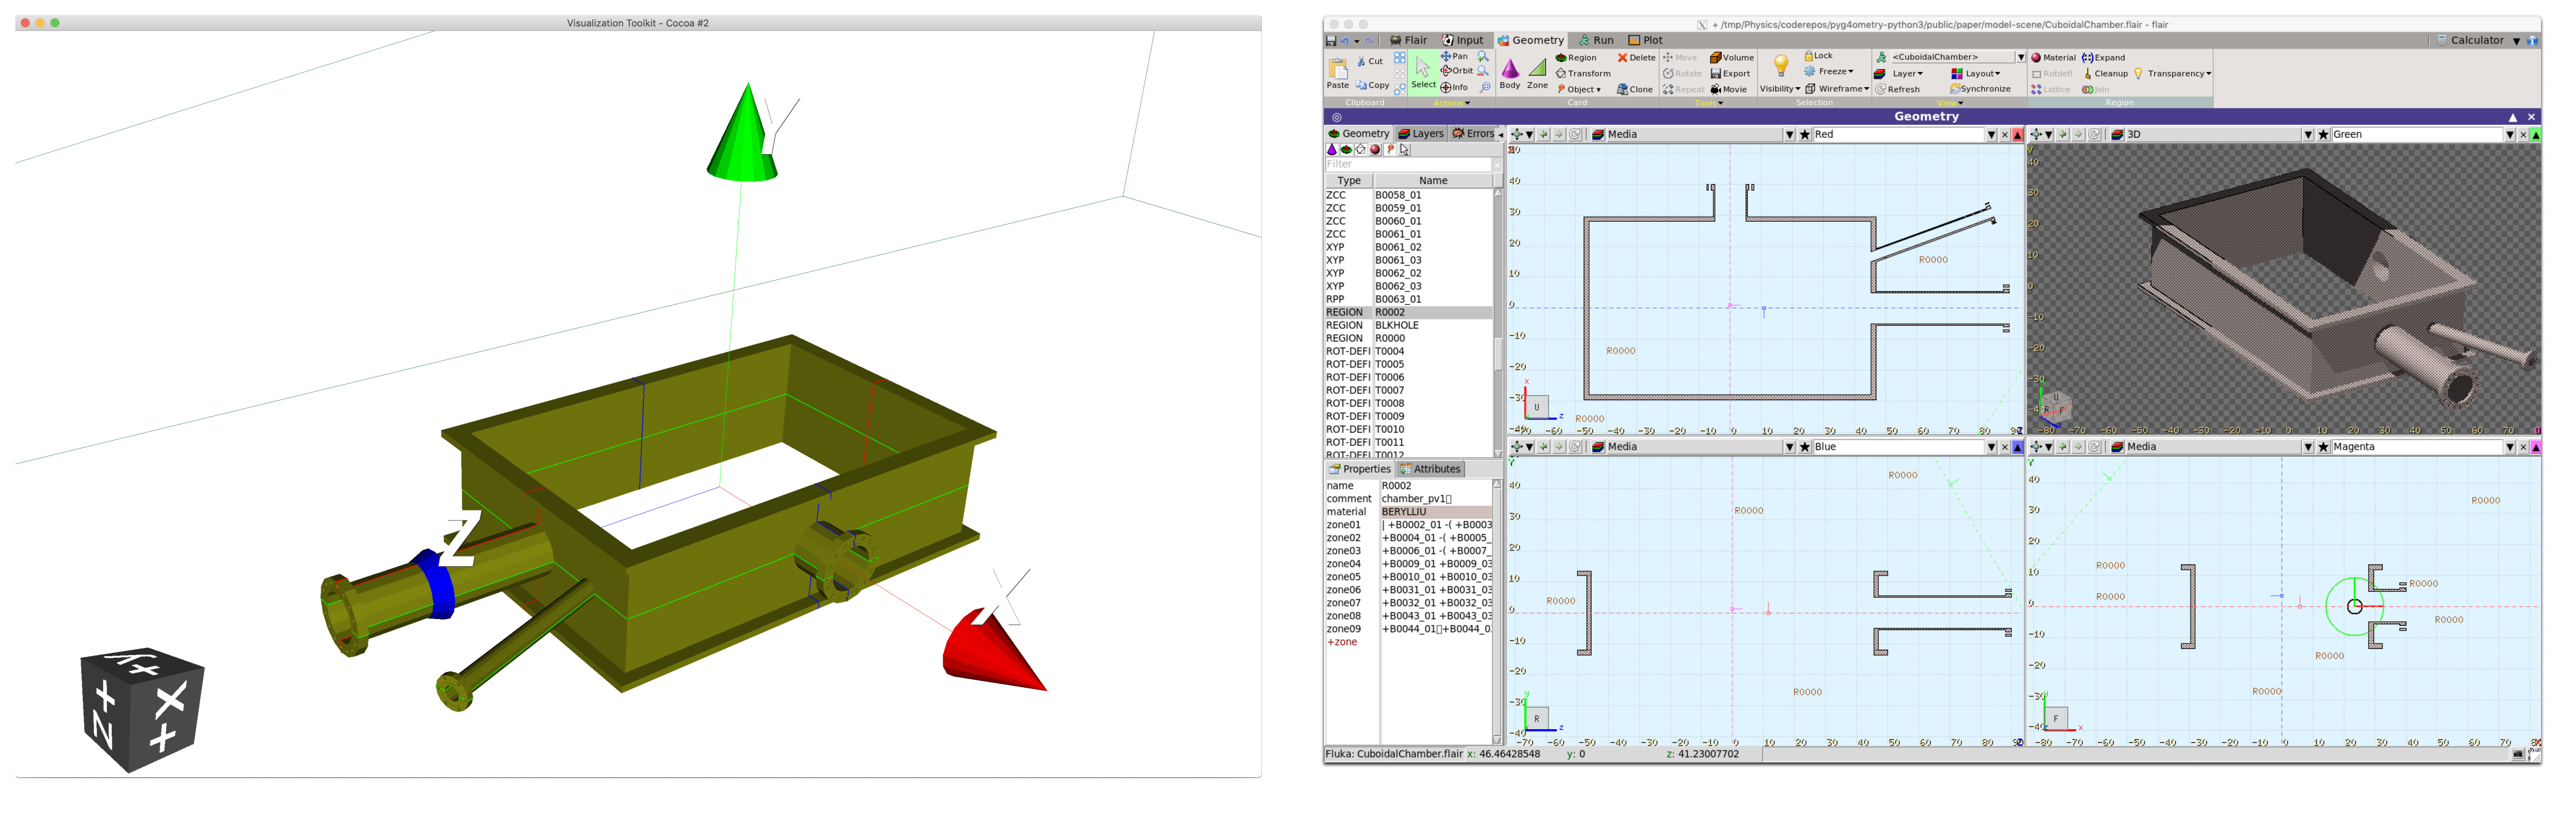
\includegraphics[width=0.9\columnwidth]{./model-scene/CuboidalChamber.pdf}
\caption{Example conversion of a simple GDML geometry to FLUKA, above:
the original model in \PYGEOMETRY{}, below: the converted FLUKA geometry
viewed in flair. The example is a sector bend dipole electromagnet.}
\label{fig:gdml-flair}
\end{center}
\end{figure}

\begin{table}[hbt!]
\centering
\begin{tabular}{ l  l  } \hline
Geant4 solid			& FLUKA region construction		\\ \hline
Box					& +2 XYP + 2 XZP + 2 YZP 		\\
Tube					& +ZCC - 2 PLA -2 XYP - ZCC	 	\\
CutTube				& +ZCC - 4 PLA -ZCC			\\
Cone				& +TRC - TRC - 2 PLA 			\\
Para					& + 6 PLA						\\
Trd					& + 6 PLA						\\
Trap					& + 6 PLA						\\
Sphere				& +SPH - SPH  - 2 PLA - 2 TRC	\\
Orb					& +SPH						\\
Torus				& +$N$ ZCC  - $N$ PLA			\\
Polycone				& +$N$ TRC -2 PLA				\\
Polyhedra				& +$N$ PLA					\\
Eltube				& +ZEC  - 2 XYP				\\
Ellipsoid				& +ELL - 2 XYP		 			\\
Elcone				& +QUA - 2 XYP				\\
Paraboloid			& +QUA - 2 XYP				\\
Hype					& +QUA - QUA - 2 XYP			\\
Tet					& +4 PLA						\\
Xtru					& +$N$ PLA \\
TwistedBox			& +$N$ PLA					\\
TwistedTtap			& +$N$ PLA					\\
TwistedTrd			& +$N$ PLA				 	\\
TwistedTube			& +$N$ PLA					\\
Arb8					& +$N$ PLA					\\
Tessellated			& +$N$ PLA				 	\\
Union				& $R_1 \cup R_2$				\\
Subtraction			& $R_1 - R_2$					\\
Intersection			& $R_1 \cap R_2$				\\
MultiUnion			& $R_1 \cup R_2 \cup R_3 \cup$	\\ \hline
\end{tabular}
\label{tab:geant2fluka}
\caption{GDML/Geant4 solids and the mapping to FLUKA regions.}
\end{table}

There are some important issues which must be considered to perform an accurate conversion. 
A Geant4 logical volume solid might need to be created from a FLUKA region composing of many zones, 
so $R_1 = +z_1\: | +z_2$, similarly a void is required to locate daughter volume placements which again 
might also be converted to a region of multiple zones $R_2= +z_3 \: | +z_4$. So creating the FLUKA region is then 
\begin{eqnarray}
R_1 - R_2 	& = & (+z_1 \: | +z_2) - ( +z_3 \: | +z_4) 			\\
			& = & (+z_1 - z_3 - z_4) \;  | \; (+z_2 - z_3 - z_4)	
\label{eqn:setDiff}
\end{eqnarray}
Geant4 has the Boolean solids associated with difference, union and intersection, so in addition to 
Equation~\ref{eqn:setDiff}, both $R_1 \cup R_2$ and $R_1 \cap R_2$ is required in FLUKA notation, so 
\begin{eqnarray}
R_1 \cup R_2 	& = & (+z_1 \: | +z_2)  \cup ( +z_3 \: | +z_4) \\
			& = & +z_1 \: | +z_2 |  +z_3 \: | +z_4
\label{eqn:setUnion}
\end{eqnarray}
and 
\begin{eqnarray}
R_1 \cap R_2 	& = & (+z_1 \: | +z_2) \cap ( +z_3 \: | +z_4) \\
			& = & +z_1 +z_3  \; | +z_1 +z_4 \; | +z_2 +z_3 \; | +z_2 +z_4
\label{eqn:setIntersection}
\end{eqnarray}

FLUKA (apart from the \fluka{lattice} directive) has no sense of a volume hierarchy. Each body is placed with a 
translation, rotation, expansion geometry directives in global coordinates. A transformation from world 
coordinates to a physical volume is built up by applying recursively daughter volume transformations 
and  this is used to place FLUKA bodies. This  in practice is very similar to the procedure to create the 
VTK visualisation already described in Section~\ref{sec:visualisation}.

In FLUKA every single space point needs to be associated with one and only one region. There is problem 
when converting Geant4 logical volumes to FLUKA regions, as the logical volume outer solid $S_{\rm logical}$ 
need to have the daughter  solids $S_{{\rm daughter},i}$ subtracted. So a solid which can be converted 
to a region $S_{\rm region}$ is then 
\begin{equation}
S_{\rm region} =  S_{\rm logical} - S_{\rm daughter,1} - S_{\rm daughter,2} - S_{\rm daughter,3} \ldots 
\label{eqn:logicalSubtraction}
\end{equation} 
If a logical volume has  number of daughter volumes which are also possibly Boolean solids, then computing 
$S_{\rm region}$ can become very complex because of Equations \ref{eqn:setDiff}, \ref{eqn:setUnion} and 
\ref{eqn:setIntersection}. 

Figure~\ref{fig:gdml-flair} shows an example conversion from GDML to FLUKA. The example is a 
vacuum chamber with three ConFlat flange (CF) beam pipes connected to CF flanges. The top and bottom plates 
have been removed to display the geometry more clearly. The model is formed of \verb|G4Box| and
\verb|G4Tubs| and Boolean operations of subtraction, intersection and union.

\subsection{Non-Convex solid decomposition}
In general the BREP solids used by Geant4 include non-convex solids, such as  Polycone, Xtru, and Twisted.  These 
particular solids are problematic when converting them to a FLUKA-readable format, as non-convex solids 
can only be created by the union of convex zones. There are two groups which need to considered, firstly those 
where 2D polygonal section needs to be decomposed these include Polycone, Polyhedron and Xtru, secondly 
those where three dimensional convex decomposition is required  TwistedBox, TwistedTrap, TwistedTrd, 
TwistedTube and Tessellated. The second classification of non convex solids are converted to CGAL 
Nef polyhedra~\cite{cgal:hk-bonp3-20b} and decomposed to convex polyhedra~\cite{cgal:h-emspe-20b}.

\subsection{Disjunctive normal form and degenerate surfaces}
Typically FLUKA will decompose a region into disjunctive normal form (DNF), this normal form is 
characterised as the union of intersections, so 
\begin{equation}
R = z_1 \; | \;z_2\;  | \; z_3 	\; | \; z_4 \dots
\end{equation}
Defining regions in terms of DNF allows the rapid test if a point is inside. Testing each zone 
$z_i$ of $R$ can terminate if a point is determined to be inside any of the convex zones $z_i$. In general 
Equation~\ref{eqn:logicalSubtraction} does not have the form of a DNF. If there are many levels of logical-physical volume 
placement, then recursive application of  Equation~\ref{eqn:logicalSubtraction} will create a nested set of 
parentheses. There are some conditions where a general Boolean expression can yield an exponential 
explosion of the final DNF. There are well known algorithms to convert logical expressions to a DNF. 
\PYGEOMETRY{} can simplify parentheses from a region by creating a SymPy~\cite{10.7717/peerj-cs.103} 
expression and using its \verb|logical| module \verb|to_dnf| method based on the Quine–McCluskey algorithm~\cite{6769983}. 
Before version 4.0 FLUKA  would simplify all regions to DNF and some converted geometry would generate 
too many zones and would fail. FLUKA version 4 allows control of the DNF expansion.

\subsection{Materials}
\PYGEOMETRY{} converts GDML/Geant4 materials to FLUKA \verb|MATERIAL| and \verb|COMPOUND| cards.
Geant4 has a class \cpinline{G4Material} to assign material state (density, physical state, temperature and pressure) 
to a logical volume. \cpinline{G4Material} has two main constructors, the first where an atomic number is supplied and 
the second is when \cpinline{G4Element} instances and relative atomic or mass abundances are provided. The {\em simple}
\cpinline{G4Material} is converted to a \fluka{material} card, whilst the {\em element} \cpinline{G4Material}  is converted to a 
\fluka{compound} card. A similar issues existing when converting \cpinline{G4Element} to FLUKA, as \cpinline{G4Element}
can either be simple, so defined only by atomic number and mass or composite and defined by a admixture defined by 
relative abundances of \cpinline{G4Isotope}. A similar mapping is performed so if an \cpinline{G4Element} is simple it is 
directly converted to a FLUKA \fluka{MATERIAL} card, and the {\it isotope} \cpinline{G4Element} is converted to a \fluka{compound}
card. Geant4 also defines a set of standard materials \cite{Geant4MaterialDB} or compounds from the US National Institute 
of Standards and Technology (NIST), so a user can, for example, just
specify the name \pyinline{G4_STAINLESS-STEEL} and \PYGEOMETRY{}  contains a matching database and creates the appropriate FLUKA 
cards during the conversion. This database is updated by running a small Geant4 program to output the appropriate
material data.

\subsection{Discussion}
Overall the conversion to FLUKA input format from GDML is quite 
advanced and stable. Relatively large experimental simulations 
have been converted from GDML to FLUKA and have been producing 
simulation results. The conversion described still requires a user to
understand how geometry is specified in both Geant4 and FLUKA. For 
example the subtraction of many non-primitive body daughter volumes from 
a mother will create a very complex non-DNF region which is inefficient when viewed in 
flair and used for simulation in FLUKA. A geometry designer can avoid this by
restricting daughter volumes solids in Geant4 that can be expressed in DNF simply,
for example a cuboid.  If \PYGEOMETRY{} is used during the creation of
 geometry then multiple codes can be targeted without additional user effort. 
There are still a few outstanding technical issues with the conversion, which are discussed 
in this section.

Currently replica, division and parametrised placements are not implemented 
and will be added in a future release. In Geant4 it is possible to create scaled 
solids or placements with reflections, so called scale in Geant4. FLUKA 
roto-translations do not support reflections and implementing reflections 
require transformation of the body definitions. This is not yet implemented 
in the current version of \PYGEOMETRY{}. 

In general, recursive application of Equations \ref{eqn:setDiff},
\ref{eqn:setUnion}, \ref{eqn:setIntersection} and \ref{eqn:logicalSubtraction} 
can result in very complex regions when converting from Geant4/GDML to 
FLUKA. The complexity of the final region expression can be compounded 
if transformed to DNF. The final region Boolean expression can be simplified by 
evaluating using the meshes for the surfaces, only retaining terms which 
do not evaluation to a null mesh.

It is possible given the GDML to FLUKA conversion algorithm described 
in this paper that coplanar overlaps exist in the FLUKA geometry.  In 
Geant4 there is no connection between surfaces used to specify on 
logical volume solid and another logical volume solid. So for example 
if a logical volume solid shared a face with one its daughter volume 
solids the body would be duplicated in the final FLUKA file. It 
is possible to remove obvious degeneracies but this is complicated by 
placements of bodies. It should be possible to cast FLUKA bodies 
{\em without} roto-translations into a {\em normal form} which can be used 
to test for approximate equality. Approximate equality is required as 
multiple application roto-translations will accrue numerical rounding errors.
An simple example of this is the XYP and PLA, it simple to transform an 
XYP into a PLA with an appropriate rotation. This would allow for the removal 
of degenerate surfaces removing potential coplanar overlaps and also reduce 
the final converted file size.

The twisted primitives need to be decomposed 
into a union of convex solids. This decomposition does not always 
succeed or produces a far from optimal number of convex solids. 
An alternative to implement these solids is to approximate each 
layer of the twisted solid as a union of tetrahedra. A similar problem 
exists for general tessellated solids, which in general
are non-convex and need decomposition into convex hulls. A potential 
way to avoid a computationally expensive decomposition step is to 
create a region formed from the unions of tetrahedra. There are numerous 
algorithms for tetrahedralisation of surface meshes in both CGAL and TetGen 
and will be implemented in a future release. Even if a stable and general 
method for converting tessellated solids exists it not efficient to define 
tessellated objects in this way and memory, body or zone limits might
be reached in FLUKA and so limit the size of CAD or STL models which 
might be loaded.

\section{STL and CAD to GDML conversion}
STL and CAD conversion are closely related. In both cases the solid 
(in the case of STL) and solids (in the case of CAD) are converted to 
tessellated solid(s). STL is a relatively simple file format that can
be loaded using pure Python. As STL files typically only contain a single 
solid the \pyinline{stl.Reader} provides a single solid and not a logical volume
as with the other file readers.
%
\begin{figure}
\begin{center}
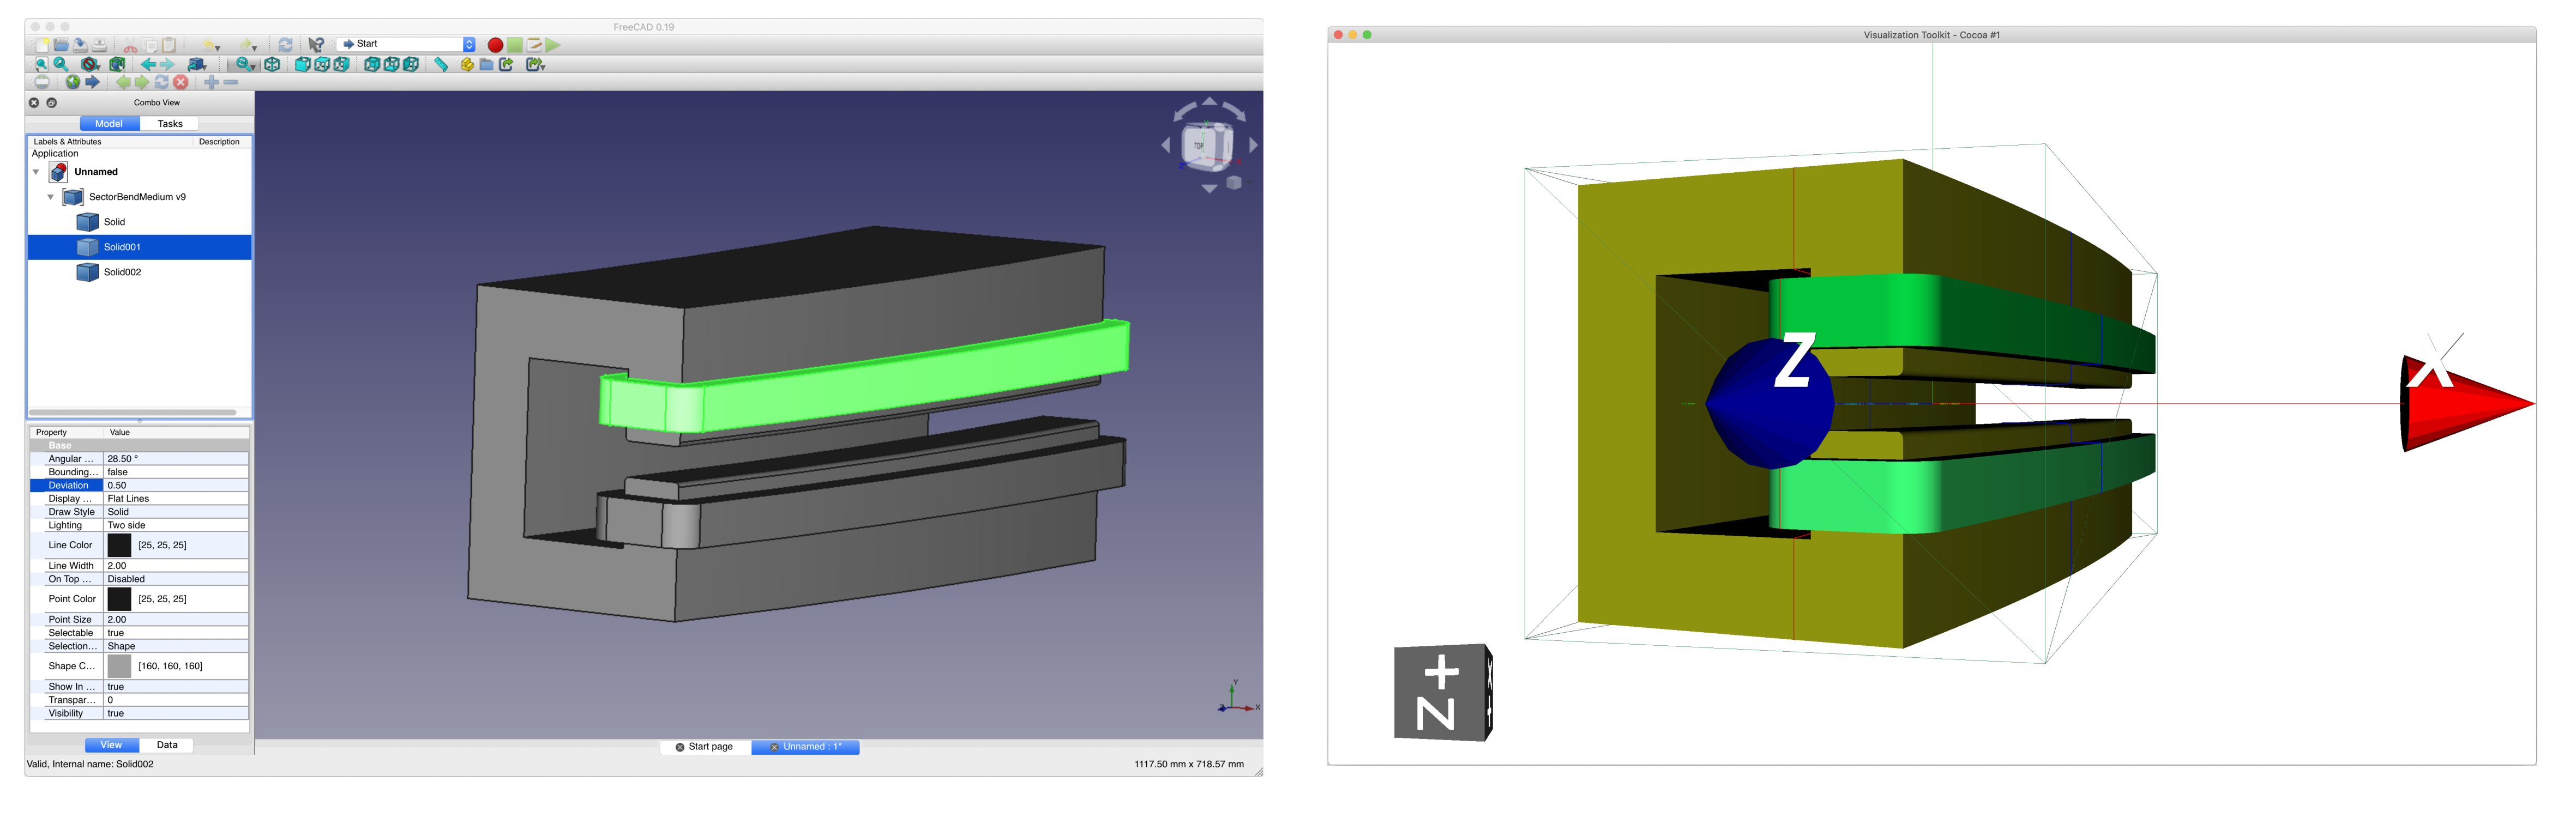
\includegraphics[width=0.9\columnwidth]{./model-scene/SectorBend.pdf}
\caption{Example conversion of a simple CAD (STEP) geometry (sector bend
  dipole electromagnet) to GDML, above: the original model in FreeCAD,
  below: the GDML geometry viewed in \PYGEOMETRY{}. }
\label{fig:cad-gdml}
\end{center}
\end{figure}

STEP and IGES files can be loaded into \PYGEOMETRY{}, via an interface 
based on FreeCAD. FreeCAD is an open source CAD/CAM program, which 
in turn is based on OpenCASCADE. FreeCAD allows for scripting in Python 
and acts as a simple to use interface to OpenCASCADE.  A STEP CAD file 
could be considered as a hierarchical tree of parts and \emph{part assemblies}, 
where a part assembly is a collection of \emph{part features}. A part feature can be used 
to create a triangular mesh which can be used to create a \PYGEOMETRY{} tessellated solid. The placement 
of the part feature is extracted from the STEP file and used to create an 
appropriate physical volume. Assignment of materials and visualisation 
attributes must be performed by  the user after conversion to GDML as rarely 
will CAD/CAM packages included the detailed information required for MCRT 
codes. Listing~\ref{lst:pythonCADLoading} shows 
how \PYGEOMETRY{} can load step files.
\begin{lstlisting}[caption={A simple \PYGEOMETRY{} Python script to load a STEP file.},label={lst:pythonCADLoading}, language=Python]
    reader = pyg4ometry.freecad.Reader("CadFileName.step")
    reader.relabelModel()
    reader.convertFlat()
    logical = reader.getRegistry().getWorldVolume()
\end{lstlisting}
Compared to other file readers, two additional steps are required \pyinline{relabelModel} and \pyinline{convertFlat}. CAD model 
part names can contain characters which are not allowed in Python dictionaries so need to be replaced by \pyinline{relabelModel}. 
CAD models might also have a hierarchy of parts and assemblies, these are converted without this structure by \pyinline{convertFlat}.
In general there is no requirement to avoid geometric overlap  of parts in a CAD file. This will result in overlaps of the solids in 
the converted tessellated solids. This is avoided by shrinking each solid, this is done by computing the a normal ${\bf n}$  for each 
vertex ${\bf v}$ and shifting its position by $\epsilon {\bf n}$, so the new vertices are ${\bf v} - \epsilon {\bf n}$. The degree of shrinking 
is user controllable. 

An example geometry representing a dipole electromagnet, consisting of three parts was created in Autodesk Fusion 360
and saved as a STEP file, \PYGEOMETRY{} produces the output in Figure~\ref{fig:cad-gdml}.

\section{Complete simulation example}
\PYGEOMETRY{} is designed to be as flexible as possible and offer the user a wide range of usage styles, input files 
and workflows. A fictitious beam line was created to demonstrate the capabilities of \PYGEOMETRY, this creates a composite 
\emph{scene} which consists of the different examples presented in this paper. The beam line consists of a vacuum chamber 
(modelled in \PYGEOMETRY{}), a vacuum gate value (STL from the manufacturer), a triplet of quadrupole magnets (exported 
from BDSIM), a sector bend dipole electromagnet (created in Autodesk Fusion 360) and finally a Faraday cup (modelled in 
flair). Each different file is loaded using \PYGEOMETRY{} reader class and the placed as a physical volume. The final composite 
geometry is shown in Figure~\ref{fig:model}. It must be noted when this complete geometry is written to GDML and loaded into 
Geant4 it cannot be visualised in anything but the ray tracer because of limitations in the OpenGL visualisation in Geant4. Another 
important note is that this geometry cannot be converted to FLUKA as it contains tessellated solids (both the STL gate valve and
dipole magnet). 
%
\begin{figure*}
\begin{center}
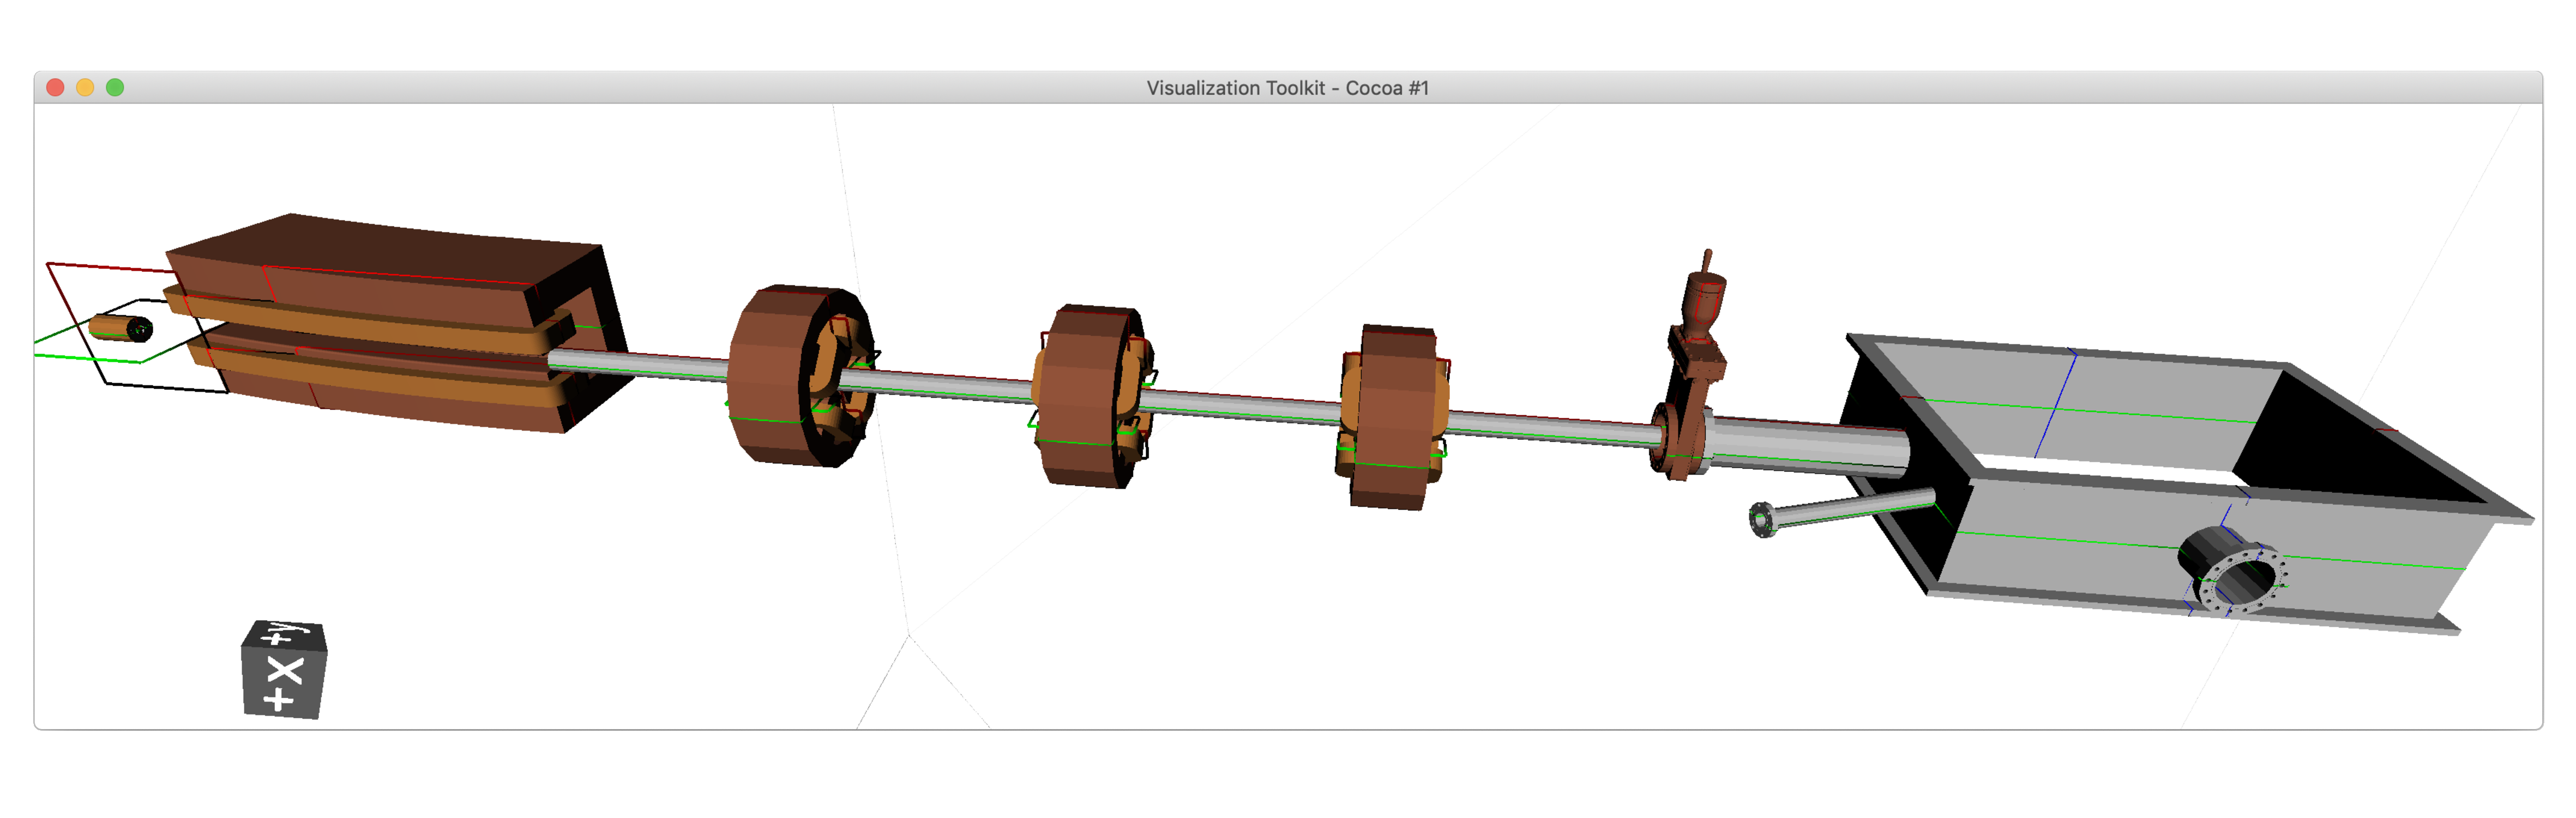
\includegraphics[width=1.0\textwidth]{./model-scene/model.pdf}
\caption{Complete compositing example using \PYGEOMETRY{}.}
\label{fig:model}
\end{center}
\end{figure*}

Having geometry wrapped in a suitable API allows a wide range of processes to be performed simply and potentially 
programmatically if it must be performed for large numbers of objects. The processes include; 
\begin{enumerate}
\item merging registries, 
\item removing volumes (de-featuring),
\item editing solid parameters,
\item replacing logical volume materials 
\item converting logical volumes to assembly volumes.
\end{enumerate}
The merging of registries and removing volumes is required to create the example shown in Figure~\ref{fig:model}. 
Each sub-component is stored in a separate registry and these have to combined without any GDML tags clashing. 
The FLUKA to GDML conversion creates logical volumes which are not generally required in Geant4, so for example
the air surrounding the Faraday cup, which is needed to specify a FLUKA geometry is converted to GDML but can be 
safely removed. Examples of other workflows or geometry manipulation processes can be found in 
the \PYGEOMETRY{} online manual.

\section{Quality assurance}
The source and manual code for \PYGEOMETRY{} is stored in a git repository (\url{https://bitbucket.org/jairhul/pyg4ometry}), 
where a public issue tracker for users is hosted to report problems or bugs with the code. The manual is created using Sphinx a 
Python documentation generator (\url{http://www.pp.rhul.ac.uk/bdsim/pyg4ometry/}). \PYGEOMETRY{} uses mature packages 
available for Python as dependencies. \PYGEOMETRY{} has  two submodules that require compilation \pyinline{pyg4ometry.pycsg} 
and \pyinline{pyg4ometry.pycgal} in C/C++. \PYGEOMETRY{}, package dependencies and extensions are installed using 
\pyinline{setuptools}. All aspects of \PYGEOMETRY{} are routinely checked using unit tests, of which 543 tests are available 
for the code, which have 84\% coverage. The unit tests also serve as minimal examples to help users understand the code operation.

\section{Conclusions and discussion}
The authors believe that tools to quickly create, either ab initio or by conversion geometry usable in Monte Carlo
particle transport programmes will save significant amounts of user effort and ultimately 
yield more accurate simulations. \PYGEOMETRY{} is a relatively complete implementation of a geometry 
creation tool, whilst heavily internally based on Geant4 and GDML, it can have utility for users of all MCRT 
codes. \PYGEOMETRY{} can clearly be extended to other formats or applications. Presently it provides a coherent and 
uniform interface to existing tools and utilities, also by using the Python programming language \PYGEOMETRY{} 
allows the programmatic control of geometry creation or modification. This approach allows the integration of 
other available tools \cite{DavisNIMA915-65} into an unified workflow.

Users should be aware of {\bf issues} with \PYGEOMETRY{}. The conversions between CAD/STL, GDML, and FLUKA 
cannot be considered bidirectional. For example Geant4 tessellated cannot be converted easily to FLUKA which does not 
have a convenient way of representing this geometry. In general a user would be unwise to attempt to convert a very large 
geometry from one format to another, but concentrate on smaller conversions of constituent parts. Workflows should focus 
on conversion from a primary format and then create conversions to another format as the need arises. This paper outlines 
the creation of geometry using \PYGEOMETRY{}, that geometry is loaded into Geant4, flair and FLUKA but detailed 
studies of the MCRT simulation performance is beyond the scope of this publication and will be addressed in the future.

There are many output format extensions that can be considered for \PYGEOMETRY{}. 
Geant4 geometry is primarily created by writing C++ programmes, so a output writer that 
converts the \PYGEOMETRY{} in memory representation to C++ will allow rapid geometry 
modelling but . This is not implemented in the current version but could be relatively quickly implemented
for users that require this functionality. At present \PYGEOMETRY{} supports reading and writing. 
Geant4 and FLUKA type files but could be extended without significant effort to other MCRT codes 
like MCNP. 

There are more complex extensions that can be considered for inclusion into \PYGEOMETRY{}.
The meshes created by \PYGEOMETRY{} are generally of very high quality and can be used for a 
wide range of applications. An idea already being developed is the export of the geometry mesh data to
data formats used in augmented or virtual reality software to create interactive visualisations of MCRT 
simulations.  Triangular meshes also have application  for GPU accelerated photon tracking in 
liquid noble dark matter detectors. Paraview/VTK are becoming standard software for complex 3D visualisation and 
the ability to write geometry to formats readily loaded and manipulated by these programs will 
significantly aid the presentation of geometry along with the results of the MCRT simulations.

\PYGEOMETRY{} is principally a toolkit but various visualisation and user interface extensions would 
significantly aid geometry creation workflows. A graphical user interface (GUI) so a user could create 
geometry without any programming knowledge would expand the number of potential users. \PYGEOMETRY{}
has been designed to interface with a GUI in a relatively straightforward manner. The VTK visualiser currently 
limits the display of very large models as geometry instances are replicated opposed to reused in visualisation. 

The conversion which would most dramatically enhance the creation of geometry is CAD to Geant4/FLUKA
without use use of a triangular or tetrahedral mesh. There are methods to decompose BREP solids to Geant4 and 
FLUKA like CSG geometry \cite{WangNuclSciTech31-82-2020, LuFusionEngineeringAndDesign124-2017}. 
The FreeCAD/OpenCASCADE interface combined with the Geant4 and FLUKA Python API present in \PYGEOMETRY{} 
will allow for the creation of CAD BREP decomposition algorithms.

There is a strong relationship between \PYGEOMETRY and Geant4 and to a lesser extent between 
\PYGEOMETRY{} and FLUKA. \PYGEOMETRY{} can be used to a testing ground for ideas prior to 
implementation in Geant4 or flair. An example of this the VTK visualisation system implemented in 
\PYGEOMETRY{}, which could be used in Geant4 to rendering of Boolean solids which frequently 
fail in the Geant4 OpenGL viewer. This would involve using CGAL meshing in the \pyinline{G4Polyhedron}
class. %There is also

\PYGEOMETRY{} is already proving to be a useful tool for geometry conversion, creation and manipulation.
There are numerous international researcher and research groups already using the code for their particular applications.
The users are focused in accelerator physics, but \PYGEOMETRY{} could find application in any scientific
area where MCRT simulations are needed, for example particle physics, space environment and medical physics.
The authors welcome contributions, extensions and bug-fixes as well a suggestions for larger collaborations.

\section{Acknowledgements}

The development of \PYGEOMETRY{} has received funding from Science and
Technology Research council grant ``The John Adams Institute for
Accelerator Science'' ST/P00203X/1 through the John Adams Institute at
Royal Holloway, and Royal Holloway Impact Acceleration Account.  Multiple
undergraduate and masters students have contributed to the code for their
degree project work, Simon Williams, Benjamin Shellswell, Joshua Albrecht.
STB has benefited from discussions with and insight of Vasilis Vlachoudis
(CERN) on FLUKA geometry and Flair.  Cédric Hernalsteens (ULB/CERN) and
Alistair Butcher (RHUL) also made useful contributions to the code.

%% The Appendices part is started with the command \appendix;
%% appendix sections are then done as normal sections
%% \appendix

%% \section{}
%% \label{}

%% References
%%
%% Following citation commands can be used in the body text:
%% Usage of \cite is as follows:
%%   \cite{key}         ==>>  [#]
%%   \cite[chap. 2]{key} ==>> [#, chap. 2]
%%

%% References with bibTeX database:

\bibliographystyle{elsarticle-num}
\bibliography{pyg4ometry}
%% Authors are advised to submit their bibtex database files. They are
%% requested to list a bibtex style file in the manuscript if they do
%% not want to use elsarticle-num.bst.

%% References without bibTeX database:

% \begin{thebibliography}{00}

%% \bibitem must have the following form:
%%   \bibitem{key}...
%%

% \bibitem{}

% \end{thebibliography}


\end{document}

%%
%% End of file 